\documentclass[a4paper,twoside,DIV15,BCOR12mm]{scrbook}

\usepackage{mathe}
\usepackage{saetze-baeuerle}
\usepackage{faktor}
\usepackage{enumerate}
\usepackage{tikz}
\usepackage{german}

\usepackage{remreset}
\makeatletter
\@removefromreset{section}{chapter}
\makeatother

\newcommand{\cF}{\mathcal{F}}

\author{Die Mitarbeiter von \url{http://mitschriebwiki.nomeata.de/}}
\title{Stochastische Prozesse}
\makeindex

\begin{document}
\maketitle
 
\newenvironment{enuma}{%
\begin{enumerate}[\hspace{1em}a)]%
}{%
\end{enumerate}%
}

\newenvironment{enumi}{%
\begin{enumerate}[\hspace{1em}i)]%
}{%
\end{enumerate}%
}

\renewcommand{\thechapter}{\arabic{chapter}}
%\chapter{Inhaltsverzeichnis}
\stepcounter{chapter}
%\renewcommand{\tocname}{bla}
\addcontentsline{toc}{chapter}{\protect\numberline {\thechapter}Inhaltsverzeichnis}
\tableofcontents

 % Vorwort

\chapter{Vorwort}
%\addcontentsline{toc}{chapter}{Vorwort}

\section*{Über dieses Skriptum}
Dies ist ein Mitschrieb der Vorlesung \glqq Stochastische Prozesse\grqq\ von Prof. Dr. Bäuerle im
Sommersemester 08 an der Universität Karlsruhe (TH).
Die Mitschriebe der Vorlesung werden mit ausdrücklicher Genehmigung von Prof Dr. Bäuerle hier veröffentlicht,
Prof. Dr. Bäuerle ist für  den Inhalt nicht verantwortlich.
\section*{Wer}
Gestartet wurde das Projekt von Joachim Breitner.


\section*{Wo}
Alle Kapitel inklusive \LaTeX-Quellen können unter \url{http://mitschriebwiki.nomeata.de} abgerufen werden.
Dort ist ein von Joachim Breitner programmiertes \emph{Wiki}, basierend auf \url{http://latexki.nomeata.de} installiert. 
Das heißt, jeder kann Fehler nachbessern und sich an der Entwicklung
beteiligen. Auf Wunsch ist auch ein Zugang über \emph{Subversion} möglich.

\setcounter{chapter}{0}
%\renewcommand{\thesection}{{\rm\bfseries §}\arabic{section}}
\renewcommand{\thesection}{\arabic{section}}
\renewcommand{\thechapter}{\Roman{chapter}}

\chapter{Markov-Ketten mit diskretem Zeitparameter}

\section{Elementare Eigenschaften von Markov-Ketten}

Gegeben sei eine Folge von Zufallsvariablen $(X_n)$ auf dem Wahrscheinlichkeitsraum $(\Omega, \cF, P)$ mit $X_n:\Omega \to S$ wobei $S$ nicht leer, und endlich oder abzählbar unendlich ist.

\begin{definition}
Eine $S\times S$-Matrix $P=(p_{ij})$ heißt \emph{stochastische Matrix}\index{stochastische Matrix}, falls $p_{ij}\ge0$ ist und für alle $i\in S$ die Zeilensumme $\sum_{j\in S} p_{ij} = 1$ ist.
\end{definition}

\begin{definition}
Sei $P$ eine stochastische Matrix. Eine (endliche oder unendliche) Folge $X_0, X_1, X_2,\ldots$ von $S$-wertigen Zufallsvariablen heißt (homogene\footnote{kurz für zeit-homogen. Die Übergangswahrscheinlichkeiten hängen nicht vom aktuellen Zeitpunkt ab.}) \emph{Markov-Kette}\index{Markov-Kette!zeitdiskrete} mit Übergangsmatrix $P$, falls für alle $n\in \MdN$\footnote{Hier ist $\MdN=1,2,\ldots$} und für alle Zustände $i_k\in S$ mit 
\[
P(X_0=i_0,\ldots,X_n=i_n) >0
\]
gilt
\[
P(X_{n+1} = i_{n+1} \mid X_0 = i_0, \ldots, X_n=i_n) = 
P(X_{n+1} = i_{n+1} \mid X_n=i_n) = p_{i_n i_{n+1}}.
\]

Die $p_{ij}$ heißen Übergangswahrscheinlichkeiten und die \emph{Startverteilung} $\nu$ der Kette ist definiert durch $\nu(i)=P(X_0=i)$ für $i\in S$.
\end{definition}

\begin{bemerkung}
Jede Folge von unabhängigen Zufallsvariablen ist eine Markov-Kette.
\end{bemerkung}

\begin{satz}[Eigenschaften von Markov-Ketten]
$(X_n)$ ist genau dann eine Markov-Kette mit Übergangsmatrix $P$, falls gilt:
\[
P(X_k = i_k,\, 0\le k\le n) = P(X_0 = i_0)\prod_{k=0}^{n-1} p_{i_k i_{k+1}} \quad \forall n\in \MdN_0 \ \forall i_k\in S
\]
genau dann wenn gilt:
\[
P(X_k = i_k,\, 1\le k\le n \mid X_0=i_0) = \prod_{k=0}^{n-1} p_{i_k i_{k+1}} \quad \forall n\in \MdN_0 \ \forall i_k\in S\text{ mit $P(X_0=i_0)>0$}
\]
genau dann wenn gilt:
\[
P(X_k = i_k,\,m\le k\le m+n) = \prod_{k=m}^{m+n-1} p_{i_k i_{k+1}} \quad \forall m,n\in \MdN_0 \ \forall i_k\in S
\]
\end{satz}

\begin{beweis}
Zur ersten Äquivalenz. Sei $A_k \da [X_k=i_k]$, $k\in\MdN_0$.

„$\Longrightarrow$“ Induktion über $n$: $n=0$ $\checkmark$, $n\curvearrowright n+1:$ 
\begin{align*}
P(A_0A_1\ldots A_nA_{n+1}) &= P(A_0\ldots A_n)\cdot P(A_{n+1}\mid A_0\ldots A_n) \\
&= P(A_0\ldots A_n)\cdot p_{i_ni_{n+1}} && \text{(Markov-Eigenschaft)}\\
&= P(X_0=i_0)\prod_{k=0}^n p_{i_ki_{k+1}} && \text{(I.V.)}
\end{align*}

„$\Longleftarrow$“ 
\begin{align*}
P(A_{n+1}\mid A_0\ldots A_n) &= \frac{P(A_0\ldots A_nA_{n+1})}{P(A_0\ldots A_n)} \\
&= p_{i_ni_{n+1}} && \text{(Vor.)}
\end{align*}
Die weiteren Äquivalenzen sind ähnlich zu beweisen.
\end{beweis}

\paragraph{Konstruktion einer Markov-Kette.} Seien $(Y_n)$ Zufallsvariablen, unabhängig und identisch gleichverteilt (u.i.v.), in $Z$. Weiter ist $g:S\times Z\to S$ eine messbare Abbildung. Definiere die Folge $(X_n)$ mit 
\[X_0=c\in S, \quad X_n = g(X_{n-1},Y_n).\]
Die so konstruierte Folge $(X_n)$ ist eine Markov-Kette mit Werten in $S$ und Übergangsmatrix $P=(p_{ij})$ mit $p_{ij} = P(g(i,X_n),j)$.

\begin{beweis}
Die Variablen $X_0,\ldots,X_n$ hängen nur von $X_0,Y_1,\ldots Y_n$ ab, sind also unabhängig von $Y_{n+1}$.
\begin{align*}
P(X_{n+1} = i_{n+1} \mid X_k = i_k, 0\le k\le n) 
&= \frac{P(X_k = i_k,\, 0\le k\le n+1)}{P(X_k = i_k,\, 0\le k\le n)} \\
&= \frac{P(X_k = i_k,\, 0\le k\le n,\, g(i_n,Y_{n+1})=i_{n+1})}{P(X_k = i_k,\, 0\le k\le n)} \\
&= \frac{P(X_k = i_k,\, 0\le k\le n)\cdot P(g(i_n,Y_{n+1})=i_{n+1})}{P(X_k = i_k,\, 0\le k\le n)} \\
&= P(g(i_n,Y_{n+1})=i_{n+1}) \\
&= \frac{P(g(i_n,Y_{n+1})=i_{n+1})\cdot P(X_n=i_n)}{P(X_n =i_n)} \\
&= \frac{P(g(i_n,Y_{n+1})=i_{n+1}, X_n=i_n)}{P(X_n =i_n)} \\
&= P(g(i_n,Y_{n+1})=i_{n+1}\mid X_n=i_n) \\
&= P(X_{n+1} = i_{n+1} \mid X_n=i_n)
\end{align*}
\end{beweis}

\begin{bemerkung}
Umgekehrt kann zu jeder stochastischen Matrix $P$ eine Markov-Kette $(X_n)$ konstruiert werden mit $X_n=g(X_{n-1},Y_n)$, wobei $(Y_n)$ u.i.v. und o.B.d.A $Y_n \sim U[0,1]$.
\end{bemerkung}

\begin{beispiel}[Lagerhaltung]
Sei $Y_n$ die Nachfrage nach einem gelagerten Produkt im Zeitintervall $(n-1,n]$. $(Y_n)$ sei u.i.v. und $Y_n\in \MdN_0$. Die Auffüll-Politik sei eine $(z,Z)$-Politik mit $z\le Z$, $z,Z\in \MdN$, die wie folgt funktiert: Falls der der Lagerbestand zur Zeit $n\le z$ ist, dann fülle auf $Z$ auf, sonst tue nichts.

Sei $X_n$ der Lagerbestand zum Zeitpunkt $n$, $S=\MdN_0$. Es gilt
\[
X_n =
\begin{cases}
(Z - Y_n)^+, & X_{n-1} \le z \\
(X_{n_1} - Y_n)^+, & X_{n-1} > z
\end{cases}
\]
Also ist $(X_n)$ eine Markov-Kette mit Übergangsmatrix $P=(p_{ij})$ und
\[
p_{ij} = 
\begin{cases}
P( (Z-Y_n)^+ = j), & i\le z \\
P( (i-Y_n)^+ = j), & i > z
\end{cases}
\]
\end{beispiel}

\begin{beispiel}[Ruinspiel]
Zwei Spieler mit Startkapital $B\in\MdN$ Euro spielen in Runden um jeweils einen Euro, etwa mit einem Münzwurf. Spieler I gewinnt dabei mit Wahrscheinlichkeit $p$. Sei $Y_n = 1$, falls Spieler I die $n$-te Runde gewinnt, und $Y_n= -1$, falls er die $n$-Runde verliert. Wir nehmen an, dass $Y_n$ u.i.v. ist.

Wir interessieren uns für das Kapital $X_n$ von Spieler I nach der $n$-ten Runde. Damit ist der Zustandsraum $S=\{0,1,\ldots,2B\}$.

Es gilt $X_0 = B$ und
\[
X_n = 
\begin{cases}
2B, &X_{n-1} = 2B \\
X_{n-1} + Y_n, & 0 < X_{n-1} < 2B \\
0, &X_{n-1} = 0.
\end{cases}
\]
Es folgt aus der Konstruktion direkt dass $(X_n)$ eine Markov-Kette ist mit Übergangsmatrix $P=(p_{ij})$, und
$p_{00} = p_{2B,2B} = 1$ sowie
\[
p_{ij} = 
\begin{cases}
p, &j=i+1\\
1-p, &j=i-1 
\end{cases}\text{ für } 0<i<2B.
\]
% Wer lust hat: Hier skizze mit Übergangswahrscheinlichkeiten.
\begin{center}
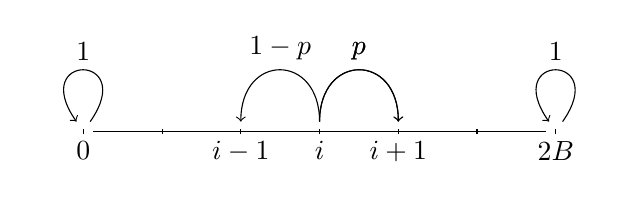
\begin{tikzpicture}
\foreach \x in {0,1,2,3,4,5,6}
	\draw (\x cm,-1pt) -- (\x cm, 1pt);
\node (null) at (0,0) {}; \draw (null) node[anchor=north] {$0$};
\node (a) at (2,0) {}; \draw (a) node [anchor=north] {$i-1$};
\node (b) at (3,0) {}; \draw (b) node [anchor=north] {$i$};
\node (c) at (4,0) {}; \draw (c) node [anchor=north] {$i+1$};
\node (zb) at (6,0) {}; \draw (zb) node [anchor=north] {$2B$};
\draw (null) -- (zb);
\draw [->] (b) .. controls +(up:1cm) and +(up:1cm) .. node [anchor=south] {$1-p$}  (a);
\draw [->] (b) .. controls +(up:1cm) and +(up:1cm) .. node [anchor=south] {$p$}  (c);
\draw [->] (b) .. controls +(up:1cm) and +(up:1cm) .. node [anchor=south] {$p$}  (c);
\draw [->] (null) .. controls +(0.7,1) and +(-0.7,1) .. node [anchor=south] {$1$}  (null);
\draw [->] (zb) .. controls +(0.7,1) and +(-0.7,1) .. node [anchor=south] {$1$}  (zb);
\end{tikzpicture}
\end{center}
\end{beispiel}

\begin{beispiel}[Wartesystem]
Zu jedem Zeitpunkt $n=0,1,\ldots$ können maximal $m$ Kunden bedient werden. $Y_n$ sei die Anzahl der zufällig im Zeitintervall $(n-1,n]$ eintreffenden Kunden und sei u.i.v.

Sei $X_n$ die Anzahl der zur Zeit $n$ wartenden Kunden, $S=\MdN_0$. Es gilt $X_0 = C$ und $X_n = (X_{n-1}-m)^+ + Y_n$. Also ist $(X_n)$ eine Markov-Kette mit Übergangsmatrix $P=(p_{ij})$ und $p_{ij} = P(Y_n = j-(i-m)^+)$, $i,j\in \MdN_0$.
\end{beispiel}

\begin{definition}
Sei $P$ eine stochastische $S\times S$-Matrix. Dann heißen die Elemente $p_{ij}^{(n)}$ von $P^n$ die $n$-Schritt-Übergangswahrscheinlichkeiten zu $P$. Wir definieren $P^0=E$, also $p^{(0)}_{ij}= \delta_{ij}$.
\end{definition}

\begin{satz}
Sei $(X_n)$ eine Markov-Kette mit Übergangsmatrix $P$. Dann gilt:
\begin{enuma}
\item $P(X_{n+m} = j\mid X_m = i) = p_{ij}^{(n)}$ für alle $i,j\in S$, $m,n\in\MdN_0$ mit $P(X_m=1)>0$.
\item $P(X_n = j) = \sum_{i\in S} P(X_0=i)p_{ij}^{(n)}$, $j\in S$, $n\in\MdN$.
\end{enuma}
\end{satz}

\begin{beweis}
\begin{enuma}
\item 
\begin{align*}
P(X_{n+m} =i_{n+m} , X_m=i_m) &= \sum_{i_{m+1},\ldots,i_{n+m+1}} P(X_m = i_m) \prod_{k=m}^{m+n+1} p_{i_ki_{k+1}} \\
&= P(X_m = i_m) p_{i_mi_{m+n}}^{(n)}
\end{align*}
\item 
\begin{align*}
P(X_n=j) &= \sum_{i\in S} P(X_n=j, X_0=i) \\
&= \sum_{i\in S} P(X_n = j \mid X_0 = i)\cdot P(X_0 = i) \\
&= \sum_{i\in S} P(X_0 = i) p_{ij}^{(n)}
\end{align*}
\end{enuma}
\end{beweis}

\begin{bemerkung}
\begin{enumi}
\item Wegen $p^{n+m}  = p^n \cdot p^m$ gilt: 
\[
p_{ij}^{(n+m)}  = \sum_{k\in S} p_{ij}^{(n)}p_{kj}^{(m)} \text{ für } i,j\in S
\]
Dies ist die „Chapman-Kolmogorov-Gleichung“\index{Chapman-Kolmogorov-Gleichung}.
\item Ist $X_0 \sim \nu$, so gilt $X_n \sim \nu\cdot P^n$.
\end{enumi}
\end{bemerkung}

\begin{satz}[Existenzssatz für Markov-Ketten]
Sei $\nu$ ein Wahrscheinlichkeitsmaß auf $S$ und $P$ eine stochastische $S\times S$-Matrix. Sei $X_n$ die $n$-te Projektion auf $\Omega \da S^{\MdN_0}$, also $X_n : \Omega\to S$, $n\in\MdN_0$ mit $X_n(\omega) = X_n( (i_0,i_1,\ldots) ) = i_n$.

Dann existiert ein Wahrscheinlichkeitsmaß $P$ auf $\cF = \oplus_{n=0}^\infty \mathcal P (S)$, so dass $(X_n)$ eine Markov-Kette mit Übergangsmatrix $P$ und Startverteilung $\nu$ ist, d.h:
\begin{itemize}
\item $P(X_0 = i_0)= \nu(i_0)$, $i_0\in S$
\item $P(X_{n+1} = j \mid X_n= i) = p_{ij}$, $i,j\in S$, $P(X_n=i)>0$.
\end{itemize}
\end{satz}

\begin{beweis}
Satz von Ionescu-Tulcea über die Fortsetzung von Maßen und die Existenz zufälliger Folgen.
\end{beweis}

\section{Klassifikation von Zuständen, Rekurrenz und Transienz}

In diesem Paragraphen widmen wir uns Fragestellungen wie diesen:
Welche Zustände in $S$ werden von der Markov-Kette mit Sicherheit besucht und welche nicht? Wenn sie besucht werden, wie oft? 

\begin{definition}
Sei $(X_n)$ eine Markov-Kette mit Übergangsmatrix $P=(p_{ij})$.
\begin{enuma}
\item $i\in S$ \emph{führt nach} $j\in S$ (kurz $i\rightsquigarrow j$)\index{$\rightsquigarrow$}, falls es ein $n\in \MdN$ gibt mit $p_{ij}^{(n)}>0$.

\item $i\in S$ \emph{kommuniziert} mit $j\in S$ (kurz $i\leftrightarrow j)$\index{$\leftrightarrow$} falls sowohl $i\rightsquigarrow j$ als auch $j\rightsquigarrow i$ gilt.
\end{enuma}
\end{definition}

\begin{bemerkung}
Für $i,j\in S$ sei $i\sim j$ definiert als $(i\leftrightarrow j) \vee (i=j)$. Diese Relation ist eine Äquivalentrelation auf $S$, da sie reflexiv, symmetrisch und transitiv ist.

Dies liefert uns eine Partition von $S$ mit den Äquivalenzklassen $K(i) \da \{j\in S \mid i\sim j\}$. Die Äquivalenzklasse $K(i)$ von $i$ enthält $i$ selbst und die mit $i$ kommunizierenden Zustände.
\end{bemerkung}

\begin{definition}
Sei $(X_n)$ eine Markov-Kette mit Übergangsmatrix $P=(p_{ij})$.
\begin{enuma}
\item $J\subset S$ heißt \emph{abgeschlossen}\index{abgeschlossene Zustandsmenge}, wenn es keine zwei Zustände $j\in J$ und $i\in S\setminus J$ gibt mit $j\rightsquigarrow i$.
\item Die Markov-Kette $(X_n)$ beziehungsweise die Übergangsmatrix $P$ heißen \emph{irreduzibel}\index{irreduzibel}, falls $S$ nur aus einer Klasse besteht, also für alle $i,j\in S$, $i\ne j$, gilt $i\leftrightarrow j$.
\end{enuma}
\end{definition}

\begin{beispiel}
\emph{Skizze, hier ausgelassen}
\end{beispiel}

\begin{beispiel}[Ruinspiel]
$\mbox{}$
\begin{center}
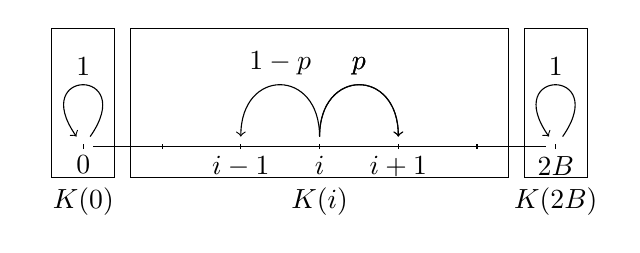
\begin{tikzpicture}
\foreach \x in {0,1,2,3,4,5,6}
	\draw (\x cm,-1pt) -- (\x cm, 1pt);
\node (null) at (0,0) {}; \draw (null) node[anchor=north] {$0$};
\node (a) at (2,0) {}; \draw (a) node [anchor=north] {$i-1$};
\node (b) at (3,0) {}; \draw (b) node [anchor=north] {$i$};
\node (c) at (4,0) {}; \draw (c) node [anchor=north] {$i+1$};
\node (zb) at (6,0) {}; \draw (zb) node [anchor=north] {$2B$};
\draw (null) -- (zb);
\draw [->] (b) .. controls +(up:1cm) and +(up:1cm) .. node [anchor=south] {$1-p$}  (a);
\draw [->] (b) .. controls +(up:1cm) and +(up:1cm) .. node [anchor=south] {$p$}  (c);
\draw [->] (b) .. controls +(up:1cm) and +(up:1cm) .. node [anchor=south] {$p$}  (c);
\draw [->] (null) .. controls +(0.7,1) and +(-0.7,1) .. node [anchor=south] {$1$}  (null);
\draw [->] (zb) .. controls +(0.7,1) and +(-0.7,1) .. node [anchor=south] {$1$}  (zb);
\draw (-0.4,-0.4) rectangle (0.4,1.5);
\draw (0,-0.4) node [anchor=north] {$K(0)$};
\draw (0.6,-0.4) rectangle (5.4,1.5);
\draw (3,-0.4) node [anchor=north] {$K(i)$};
\draw (5.6,-0.4) rectangle (6.4,1.5);
\draw (6,-0.4) node [anchor=north] {$K(2B)$};
\end{tikzpicture}
\end{center}
\end{beispiel}

\begin{lemma}
$J\subset S$ ist genau dann abgeschlossen, wenn $(p_{ij},\, i,j\in J)$ stochastisch ist.
\end{lemma}
\begin{beweis}
„$\Longrightarrow$“: Klar. „$\Longleftarrow$“: Es gilt: $(p_{ij},\, i,j\in J)$ stochastisch $\iff$ $(p_{ij}^{(n)},\, i,j\in J)$ stochastisch für alle $n\in \MdN$.
\end{beweis}

\pagebreak[2]
Sei $(X_n)$ eine Markov-Kette mit Übergangsmatrix $P=(p_{ij})$. Es sei
\[
T_i \da \inf\{n\in\MdN\mid X_n =i\}
\]
die (zufällige) Ersteintrittszeit der Markov-Kette in den Zustand $i$.

Wir setzen dabei $\inf\emptyset \da \infty$. Weiter sei für $i,j\in S$, $n\in \MdN$:
\begin{align*}
f_{ij}^{(n)} &\da P(T_j=n\mid X_0=i) = P_i(T_j=n) \\
&=P(X_n=j,\, X_\nu\ne j \text{ für } 1 < \nu < n\mid X_0=i) \\
f_{ij}^{(0)} &\da 0
\end{align*}

Offenbar ist $f_{ij}^{(1)} = p_{ij}$. Weiter definieren wir
\[
f_{ij}^{*} \da \sum_{n=0}^\infty f_{ij}^{(n)} = \sum_{n=0}^\infty P_i(T_j=n) = P_i(T_j<\infty) = P_i(\exists n\in \MdN: X_n=j)\in[0,1]
\]

\begin{definition}
Ein Zustand $i\in S$ heißt \emph{rekurrent}\index{rekurrent}, falls $f_{ii}^{*} = 1$ und \emph{transient}\index{transient} sonst. % Das sind ganz wichtige Begriffe.
\end{definition}

\begin{lemma}
\label{lem2.2}Für alle $n\in\MdN$, $i,j\in S$ gilt:
\[
p_{ij}^{(n)} = \sum_{k=1}^n f_{ij}^{(k)} p_{jj}^{(n-k)}
\]
\end{lemma}

\begin{beweis}[Methode des ersten Besuches]
Unter Verwendung der Formel $P(AB\mid C) = P(B\mid C)\cdot P(A\mid BC)$ für Ereignisse $A,B,C$ zeigen wir:
\begin{align*}
p_{ij}^{(n)} &= P_i(X_n=j) = \sum_{k=1}^n P({X_n=j},\, {X_\mu\ne j,\, 1<\mu<k,\, X_k = j}\mid {X_0=i}) \\
&= \sum_{k=1}^n P_i(X_\mu\ne j,\, 1<\mu<k,\, X_k = j)\cdot\\
&\quad\quad\quad\quad \underbrace{P(X_n=j\mid X_0=i,\,X_\mu\ne j,\, 1<\mu<k,\, X_k = j)}_{=P(X_n=j\mid  X_k=j)}\\
&=\sum_{k=1}^nf_{ij}^{(k)} p_{jj}^{(n-k)}
\end{align*}
\end{beweis}

\begin{satz}
\label{satz2.3}%
$i\in S$ ist rekurrent genau dann, wenn gilt:
\[
\sum_{n=0}^\infty p_{ii}^{(n)} = \infty
\]
\end{satz}

\begin{beweis}
Für $s\in(0,1)$ erhalten wir aus Lemma \ref{lem2.2}:
\begin{align*}
\sum_{n=0}^\infty p_{ii}^{(n)} s^n &= 1 + \sum_{n=1}^\infty p_{ii}^{(n)} s^n = \\
&= 1 + \sum_{n=1}^\infty s^n\sum_{k=1}^n f_{ii}^{(k)}p_{ii}^{(n-k)} \\
&= 1 + \sum_{k=1}^\infty f_{ii}^{(k)} s^k \sum_{n=k}^\infty p_{ii}^{(n-k)} s^{n-k} \\
&= 1 + \sum_{k=1}^\infty f_{ii}^{(k)} s^k \sum_{n=0}^\infty p_{ii}^{(n)} s^{n} 
\end{align*}

Abkürzend schreiben wir $P(s)\da \sum_{k=1}^\infty f_{ii}^{(k)} s^k$ und $F(s)=\sum_{n=0}^\infty p_{ii}^{(n)} s^{n}$, also gilt \[P(S) = 1 + F(s)\cdot P(s).\]
Nun sei $s\to 1$ (monotone Konvergenz!), und wir erhalten
\[
P(1) = 1 + P(1)\cdot f_{ii}^*.
\]
Es folgt: Ist $f_{ii}^* = 1$, so gilt $P(1) = 1 + P(1)$, also ist $P(1) = \sum_{n=0}^\infty p_{ii}^{(n)} = \infty$. Ist ansonsten $f_{ii}^{*}<1$, so gilt $P(1) = \frac1{1-f_{ii}^*} < \infty$.
\end{beweis}
%$p,P,\pi,\Pi, \mathcal P, \mathfrak P, \mathfrak p$

\begin{bemerkung}
Die im Satz \ref{satz2.3} auftretende Reihe kann wie folgt interpretiert werden:
\begin{align*}
\sum_{n=0}^\infty p_{ii}^{(n)}
= \sum_{n=0}^\infty E_i[1_{[X_n=i]}]
= \sum_{n=0}^\infty E_i[1_{[X_n=i]}]
= E(\sum_{n=0}^\infty 1_{[X_n=i]})
\end{align*}
Sie bezeichnet also die erwartete Anzahl der Besuche des Zustandes $i\in S$.
\end{bemerkung}

\begin{satz}[Solidaritätsprinzip]
Ein Zustand $i\in S$ ist rekurrent (bzw. transient), wenn jeder Zustand in $K(i)$ rekurrent (bzw. transient) ist.
\end{satz}

\begin{beweis}
Sei $i$ rekurrent und $j\in K(i)$, $j\ne i$, das heißt es gibt $n,m\in \MdN$, so dass $p_{ij}^{(m)}\cdot p_{ji}^{(n)}>0$.
Mit der Abschätzung
\begin{align*}
\sum_{k=0}^\infty p_{jj}^{(k)} 
&\ge \sum_{k=0}^\infty p_{jj}^{(m+n+k)} 
\ge \sum_{k=0}^\infty p_{ji}^{(n)} p_{ii}^{(k)} p_{ij}^{(m)}
= p_{ij}^{(m)} p_{ji}^{(n)} \sum_{k=0}^\infty p_{ii}^{(k)}
\end{align*}
und Satz \ref{satz2.3} ist $\sum_{k=0}^\infty p_{jj}^{(k)}=\infty$ und $j$ rekurrent.
\end{beweis}

\begin{bemerkung}
Ist $i\in S$ rekurrent (bzw. transient), so sagen wir $K(i)$ ist rekurrent (bzw. transient).

Ist $(X_n)$ irreduzibel, und ein $i\in S$ ist rekurrent (bzw. transient), so sagen wir $(X_n)$ ist rekurrent (bzw. transient).
\end{bemerkung}

\begin{beispiel}[Irrfahrt auf den ganzen Zahlen, „Random Walk“]
\label{bsp2.3}
Es sei $X_n=\sum_{k=1}^n Y_k = X_{n-1}+Y_k$ und $X_0=0$, wobei $(Y_n)$ u.i.v. mit \[P(Y_n=1)=p = 1 - P (Y_n=-1) =1-q,\quad p\in (0,1)\] ist ($S=\MdZ$).

\begin{center}
\begin{tikzpicture}
\foreach \x in {0,1,2,3,4,5,6}
	\draw (\x cm,-1pt) -- (\x cm, 1pt);
%\node (null) at (0,0) {}; \draw (null) node[anchor=north] {$0$};
\node (a) at (2,0) {}; \draw (a) node [anchor=north] {$i-1$};
\node (b) at (3,0) {}; \draw (b) node [anchor=north] {$i$};
\node (c) at (4,0) {}; \draw (c) node [anchor=north] {$i+1$};
%\node (zb) at (6,0) {}; \draw (zb) node [anchor=north] {$2B$};
\draw (null) -- (zb);
\draw [->] (b) .. controls +(up:1cm) and +(up:1cm) .. node [anchor=south] {$q$}  (a);
\draw [->] (b) .. controls +(up:1cm) and +(up:1cm) .. node [anchor=south] {$p$}  (c);
\draw [->] (b) .. controls +(up:1cm) and +(up:1cm) .. node [anchor=south] {$p$}  (c);
%\draw [->] (null) .. controls +(0.7,1) and +(-0.7,1) .. node [anchor=south] {$1$}  (null);
%\draw [->] (zb) .. controls +(0.7,1) and +(-0.7,1) .. node [anchor=south] {$1$}  (zb);
\end{tikzpicture}
\end{center}
Die Markov-Kette $(X_n)$ ist nach Konstruktion eine irreduzible Markov-Kette. Ist $(X_n)$ rekurrent oder transient?

Wir wenden Satz \ref{satz2.3} an und untersuchen o.B.d.A $i=0$. Es gilt für alle $n\in \MdN_0$:
\begin{align*}
p_{00}^{(2n+1)} &= 0\\
p_{00}^{(2n)} &= p^nq^n \binom{2n}{n} = p^nq^n \frac{(2n)!}{(n!)^2}
\end{align*}
\end{beispiel}

\begin{centering}
\Large Hier bitte Vorlesung vom 22.4. eintragen.
\end{centering}

\begin{centering}
\Large Hier bitte Vorlesung vom 23.4. eintragen:
\end{centering}


\section{Stationäre Verteilungen}

Sei $(X_n)$ eine Markov-Kette mit Übergangsmatrix $P$ und Startverteilung $\nu$.

Dann ist $X_n \sim \nu \cdot P^n$. Im Allgemeinen hängt diese Verteilung von $\nu$ ab. Es gibt aber spezielle Verteilungen
$\nu$, so dass die mit dieser Verteilung gestartete Kette zu jedem Zeitpunkt $n$ die selbe Verteilung $\nu$ besitzt. Man sagt dann,
die Kette ist \emph{im Gleichgewicht} bzw. \emph{stationär}.

\begin{definition}
  Eine Abbildung $\nu: S \rightarrow \MdR_{\geq 0}$ heißt \emph{Maß}.

  NB: Ein Maß $\nu$ definiert ein Maß $\mathcal{P}(S) \rightarrow \MdR_{\geq 0}, A \mapsto \sum_{a \in A} \nu(a) $ im gewöhnlichen Sinne.
  Falls $\sum_{a \in S} \nu(a) = 1$, so definiert es sogar eine Verteilung.
\end{definition}

\begin{definition}
  Sei $(X_n)$ eine Markov-Kette mit Übergangsmatrix $P = (p_{i,j})$. Ein Maß $\nu$ heißt \emph{invariant} für $P$, falls $\nu \cdot P = \nu$, d.h.
  falls gilt
  \begin{align*}
    \sum_{i \in S} \nu(i) \cdot p_{i,j} = \nu(j)
  \end{align*}
  Ist $\nu$ eine Verteilung und invariant, so nennt man $\nu$ auch \emph{stationäre Verteilung} oder \emph{Gleichgewichts-Verteilung}.
\end{definition}

\begin{bemerkung}
  a) Ist $S$ endlich, so kann jedes (nichtdegenerierte) invariante Maß zu einer stationären Verteilung normiert werden.

  b) Ist $\nu$ invariant, so gilt $\nu \cdot P^n = \nu$ ($n \in \MdN_0$).

  Ist $\nu$ eine stationäre Verteilung, so gilt
  \begin{align*}
    P_\nu(X_n = j) = \sum_{i \in S} v(i) \cdot p_{i,j}^{(n)} = \nu(j),
  \end{align*}
  d.h. die mit $\nu$ gestartete Kette hat zu jedem Zeitpunkt die Verteilung $\nu$.

  c) Ist $P$ irreduzibel und $\nu \neq 0$ ein invariantes Maß, so ist $\nu > 0$.

  Denn: $\nu \neq 0$, also existiert $i_0 \in S$ mit $\nu(i_0) \geq 0$.
  Wegen der Irreduzibilität gibt es ferner für jedes $j \in S$ ein $n \in \MdN_0$ mit $p_{i_0,j}^{(n)} \geq 0$. Zusammen:
  \begin{align*}
    \nu(j) = \sum_{i \in S} \nu(i) \cdot p_{i,j}^{(n)} \geq \nu(i_0) p_{i_0,j}^{(n)} > 0
  \end{align*}
\end{bemerkung}


Gibt es immer ein invariantes Maß bzw. eine stationäre Verteilung? Ist es eindeutig?

Im Folgenden sei $P$ irreduzibel. Wir definieren für ein beliebiges $k \in S$ das Maß $\gamma_k$ wie folgt:
\begin{align*}
  \gamma_k(i) := E_k[\sum_{n=1}^{T_k} 1_{[X_n = i]}]
\end{align*}


\begin{satz}
\label{satz3.1}
  Sei $(X_n)$ irreduzibel und rekurrenz, $k \in S$. Dann gilt:
  \begin{enuma}
  \item $\gamma_k$ ist ein invariantes Maß
  \item $0 < \gamma_k < \infty$
  \item $\gamma_k$ ist das einzige invariante Maß mit $\gamma_k(k) = 1$ (d.h. $\gamma_k$ ist eindeutig bis auf Vielfache)
  \end{enuma}
\end{satz}

\begin{beweis}
\begin{enuma}
\item Zunächst gilt:
  \begin{align*}
      \gamma_k(i)
    &= E_k[\sum_{n=1}^{T_k} 1_{[X_n = i]}]
     = E_k[\sum_{n=1}^\infty 1_{[X_n = i, n \leq T_k]}]
     = \sum_{n=1}^\infty P_k(X_n = i, n \leq T_k)\\
    &= \sum_{n=1}^\infty \sum_{j \in S} P_k(X_n = i, X_{n-1} = j, n \leq T_k)
  \end{align*}
  Für $j \neq k$ erhält man
  \begin{align*}
      &P_k(X_n = i, X_{n-1} = j, n \leq T_k)\\
    = &P_k(X_n = i, X_{n-1} = j, X_{n-2} \neq k, \ldots, X_1 \neq k, X_0 = k) / P(X_0 = k)\\
    = &P_k(X_n = i | X_{n-1} = j, X_{n-2} \neq k, \ldots, X_1 \neq k, X_0 = k) \cdot P_k(X_{n-1} = j, X_{n-2} \neq k, \ldots, X_1 \neq k)\\
    = &p_{j,i} \cdot P_k(X_{n-1} = j, n \leq T_k)
  \end{align*}
  Die so erhaltene Identität gilt auch für $j = k$, und es folgt
  \begin{align*}
    \gamma_k(i) &= \sum_{n=1}^\infty \sum_{j \in S} P_k(X_n = i, X_{n-1} = j, n \leq T_k)\\
                &= \sum_{n=1}^\infty \sum_{j \in S} p_{j,i} \cdot P_k(X_{n-1} = j, n \leq T_k)\\
                &= \sum_{j \in S} p_{j,i} \sum_{n=0}^\infty P_k(X_n = j, n+1 \leq T_k)\\
                &= \sum_{j \in S} p_{j,i} E_k[\sum_{n=0}^{T_{k-1}} 1_{[X_n = j]}]\\
                &= \sum_{j \in S} p_{j,i} E_k[\sum_{n=0}^{T_k} 1_{[X_n = j]}]
                 = \sum_{j \in S} \gamma_k(j) p_{j,i}
  \end{align*}

\item
  Nach Bemerkung c) oben gilt $\gamma_k > 0$, denn $\gamma_k(k) = 1$. Wegen $\gamma_k = \gamma_k \cdot P^n$ folgt
  \begin{align*}
    1 = \gamma_k(k) \geq \gamma_k(j) \cdot p_{j,k}^{(n)}
  \end{align*}
  für jedes $j \in S$. Es gibt allerdings mindestens ein $p_{j,k}^{(n)} > 0$, denn die Markov-Kette ist irreduzibel; daran erkennt man
  $\gamma_k < \infty$.

\item 
  Sei $\lambda$ ein weiteres, invariantes Maß mit $\lambda(k)=1$. Es gilt also:
  \begin{align*}
    \lambda(j) &= \sum_{i \in S\setminus\{k\}} \lambda(i) \cdot p_{i,j} + 1 \cdot p_{k,j}\\
               &= \sum_{i \in S\setminus\{k\}} \left( \sum_{l \in S\setminus\{k\}} \lambda(l) \cdot p_{l,i} + p_{k,i} \right) p_{i,j} + p_{k,j}\\
               &= \sum_{i,l \in S\setminus\{k\}} \lambda(l) \cdot p_{l,i} \cdot p_{i,j} + \sum_{i \in S\setminus\{k\}} p_{k,i} \cdot p_{i,j} + p_{k,j}\\
               &= \sum_{i,l \in S\setminus\{k\}} \lambda(l) \cdot p_{l,i} \cdot p_{i,j} + P_k(X_2 = j, T_k \geq 2) + P_k(X_1 = j, T_k \geq 1)
  \end{align*}
  Iterativ erhalten wir für $n \in \MdN$:
  \begin{align*}
    \lambda(j) &= \sum_{i_0, i_1, \ldots, i_n \in S\setminus\{k\}} \lambda (i_n) \prod_{r=1}^n p_{i_r,i_{r-1}} p_{i_0,j} + \sum_{r=1}^{n+1} P_k(X_r = j, T_k \geq 1)\\
               &\geq \sum_{r=1}^{n+1} P_k(X_r = j, T_k \geq 1) = E_k[\sum_{r=1}^{\min(n+1,T_k)} 1_{[X_r = j]}] \towegen{LDC} \gamma_k(j)
  \end{align*}
  Es ist also $\lambda - \gamma_k$ ebenfalls ein invariantes Maß mit $(\lambda - \gamma_k)(k) = 0$; nach Bemerkung c) folgt
  $\lambda - \gamma_k = 0$, d.h. $\lambda = \gamma_k$.
\end{enuma}

\end{beweis}

\begin{bemerkung}
\begin{enuma}
\item Ist $S$ endlich und $P$ irreduzibel, so folgt aus Satz \ref{satz3.1}, dass eine stationäre Verteilung existiert.
\item Ist $(X_n)$ irreduzibel und transient, so kann  keine stationäre Verteilung existieren, denn:

Ansgenommen es existiert eine stationäre Verteilung $\pi$. Dann ist
\begin{align*}
\pi(j) &= \sum_{i\in S} \pi(i) P_{ij}^{(n)}.
\end{align*}
Für $n\to\infty$ wird daraus (mit majorisierter Konvergenz und der bekannten Eigenschaft transienter Übergangswahrscheinlichkeiten):
\begin{align*}
\pi(j) &= \sum_{i\in S} \pi(i) \lim_{n\to\infty} P_{ij}^{(n)} \\
&= \sum_{i\in S} \pi(i) \cdot 0 \\
&= 0
\end{align*}
\end{enuma}

\end{bemerkung}

\begin{definition}
Für $i\in S$ sei
\begin{align*}
m_i \da E_i[T_i] &= \sum_{n=1}^\infty n \cdot P_i(T_i=n) + \infty \cdot (1-f_{ii}^*) \\
&= \sum_{n=1}^\infty  n\cdot f_{ii}^{(n)} + \infty \cdot (1-f_{ii}^*)
\end{align*}
die \emph{mittlere Rückkehrzeit}\index{mittlere Rückkehrzeit} des Zustands $i$.
\end{definition}

\begin{bemerkung}
Ist $j$ transient, so folgt $m_j=\infty$.
\end{bemerkung}

\begin{definition}
Ein Zustand $i\in S$ heißt \emph{positiv rekurrent}\index{positiv rekurrent}, falls $m_i<\infty$ und \emph{nullrekurrent}\index{nullrekurrent}, falls $i$ rekurrent und $m_i=\infty$ ist.
\end{definition}

\begin{bemerkung}
Jeder positiv rekurrente Zustand ist auch rekurrent.
\end{bemerkung}

\begin{satz}
\label{satz3.2}Sei $(X_n)$ eine irreduzible Markov-Kette. Die folgenden Aussagen sind äquivalent:
\begin{enumi}
\item Es existiert eine stationäre Verteilung.
\item Es gibt einen positiv rekurrenten Zustand.
\item Alle Zustände sind in $S$ positiv rekurrent.
\end{enumi}
Sind diese Bedingungen erfüllt, so ist die stationäre Verteilung eindeutig und durch \[\pi(i)=\frac 1 {m_i}\] gegeben.
\end{satz}

\begin{beweis}
\begin{enumerate}[(iii) $\implies$ (ii)]
\item[(iii) $\implies$ (ii)] $\checkmark$
\item[(ii) $\implies$ (i)] Sei $k\in S$ mit $m_k<\infty$, dann ist $(X_n)$ rekurrent und mit Satz \ref{satz3.1} ist $\gamma_k$ ein invariantes Maß. Dann gilt:
\begin{align*}
\sum_{j\in S} \gamma_k(j) 
&= \sum_{j\in S} E_k[ \sum_{n=1}^{T_k} 1_{[X_n=j]}] \\
&= E_k[\sum_{n=1}^{T_k} \sum_{j\in S} 1_{[X_n=j]}] \\
&= E_k[\sum_{n=1}^{T_k} 1] \\
&= E_k[T_k] = m_k <\infty
\end{align*}
also ist $\gamma_k$ normierbar.

\item[(i) $\implies$ (iii)] Sei $\pi$ eine stationäre Verteilung und $k\in S$. Insbesondere sind $\pi(j)>0$ für alle $j\in S$. Dann ist $\gamma \da \frac{\pi}{\pi{k}}$ ein invariantes Maß mit $\gamma(k)=1$.  Nach Satz \ref{satz3.1} c) folgt $\gamma = \gamma_k$. Beachte dass im Beweis von \ref{satz3.1} c) die Voraussetzung $(X_n)$ rekurrent nicht verwendet wurde.
Wie oben ist 
\[
m_k=\sum_{j\in S}\gamma_k(j) = \frac 1 {\pi(k)} \sum_{j\in s} \pi(j) = \frac1{\pi(k)} < \infty.\]

Da $k\in S$ beliebig ist, folgt die Behauptung (iii).

Außerdem ist gezeigt, dass $\pi(k)=\frac1{m_k}$.
\end{enumerate}
\end{beweis}
\begin{bemerkung}
\begin{enumi}
\item Es gilt also die folgende Trichotomie für irreduzible Markov-Ketten, das hießt eine irreduzible Markov-Kette gehört immer zu genau einer der folgenden Fälle:
\begin{itemize}
\item Die Markov-Kette ist transient, es gibt keine stationäre Verteilung.
\item Die Markov-Kette ist nullrekurrent, insbesondere gilt für alle $i,j\in S$:
\[P_i(T_j<\infty) = 1\text{ und }E_i[T_j]=\infty\]
und es gibt ein (bis auf Vielfache) eindeutiges invariantes Maß, aber keine stationäre Verteilung.
\item Die Markov-Kette ist positiv rekurrent, für alle $i,j\in S$ ist $E_i[T_j]<\infty$ und es gibt eine stationäre Verteilung.
\end{itemize}

\item Ist $S$ endlich und die Markov-Kette irreduzibel, so ist sie automatisch positiv rekurrent.

\item Ist $\pi$ eine stationäre Verteilung, so gilt:
\begin{align*}
\pi(i) = \frac{\gamma_k(i)}{\sum_{j\in S} \gamma_k(j)}
= \frac{E_k[\sum_{n=1}^{T_k} 1_{[X_n=i]}]}{E_k[T_k]}
\end{align*}
$\pi(i)$ ist also der durchschnittliche Bruchteil der Zeit, den die Markov-Kette im Zusatand $i$ verbringt, während sie einen Zyklus durchläuft.
\end{enumi}
\end{bemerkung}

\begin{beispiel}
Sei $S=\{1,2\}$. Die Übergangsmatrix $P$ sei gegeben durch 
\[
P=
\begin{pmatrix}
1-\alpha & \alpha \\
\beta & 1-\beta
\end{pmatrix}, \quad \alpha,\beta \in (0,1]
\]
Also ist die Markov-Kette irreduzibel und positiv rekurrent. Die stationäre Verteilung ist die Lösung des linearen Gleichungssytems
\[ \pi P = \pi\]
unter Berücksichtigung von $\pi \ge 0$ und $\pi(1) + \pi(2) = 1$,
also
\[
\pi(1) = \frac\beta{\alpha + \beta}, \quad \pi(2)=\frac{\alpha}{\alpha+\beta}.
\]
\end{beispiel}

\begin{beispiel}[Irrfahrt]
Siehe Beispiel \ref{bsp2.3}: Für $p\ne q$ ist die Markov-Kette transient. Existiert ein invariantes Maß? Ansatz:
\[
\gamma(j) = \sum_{i\in \MdZ} \gamma (i) p_{ij} = \gamma(j+1)\cdot q = \gamma(j-1)\cdot p
\]
\[
\implies \gamma(j+1) - \gamma(j) = \frac pq (\gamma(j) - \gamma(j-1)
\]
Also: $\gamma_1(j) = 1$  und $\gamma_2(j) = (\frac pq)^{j}$, $j\in \MdZ$, sind verschiedene invariante Maße.

Ist $p=q=\frac 12$, so ist die Markov-Kette rekurrent. Ist sie nullrekurrent oder positiv rekurrent? Es gibt keine stationäre Verteilung (siehe oben), die Markov-Kette ist also nullrekurrent.
\end{beispiel}

\begin{beispiel}[Geburts- und Todesprozess in diskreter Zeit]
Es sei $(X_n)$ eine Markov-Kette mit $S=\MdN_0$ und Übergangsmatrix 
\[
P = 
\begin{pmatrix}
p_{00} & p_{01} & 0 & \cdots \\
p_{10} & p_{11} & p_{12} & 0 & \cdots \\
0 & p_{21} & p_{22} & p_{23} & \ddots \\
\vdots & 0 & p_{32} & p_{33}  & \ddots \\
 & \vdots &\ddots & \ddots & \ddots  & 
 \end{pmatrix}
\]
mit $p_{01}>0$, $p_{i,i+1}>0$, $p_{i,i-1}>0$ für alle $i\ge 1$, also ist $(X_n)$ irreduzibel. Wan ist $(X_n)$ positiv rekurrent? 

Der Ansatz $\pi P=\pi$ liefert:
\begin{align*}
\pi(0) &= p_{00} \cdot \pi(0) + p_{10}\cdot \pi(1) \\
\pi(i) &= p_{i-1,i}\cdot \pi(i-1) + p_{ii}\cdot \pi(i) + p_{i,i+1}\cdot\pi(i+1) \\
\iff p_{i,i-1}\cdot \pi(i) + p_{i,i+1} \pi(i) &= p_{i-1,i}\cdot \pi(i-1) + p_{i+1,i} \cdot \pi(i+1) \\
\iff p_{i+1,i}\cdot \pi(i+1) - p_{i,i+1}\cdot \pi(i) &= p_{i,i-1}\cdot \pi(i) - p_{i-1,i}\cdot \pi(i-1) \\
&= \ldots = p_{10}\cdot\pi(1) - p_{01}\cdot\pi(0) \\
\intertext{Aus der ersten Gleichung folgt $p_{01}\cdot\pi(0) = p_{10}\cdot\pi(1)$ und damit:}
p_{i+1,i}\cdot \pi(i+1) - p_{i,i+1}\cdot \pi(i) &= 0 \\
\implies \pi(i+1) &= \frac{p_{i,i+1}}{p_{i+1,i}} \pi(1) \\
&= \ldots = \pi(0) \cdot \prod_{k=1}^i \frac{p_{k,k+1}}{p_{k+1,k}}
\end{align*}
Für $\pi(0)>0$ erhält man ein invariantes Maß. $(X_n)$ ist positiv rekurrent, falls 
\[
\sum_{i=1}^\infty \prod_{k=0}^i \frac{p_{k,k+1}}{p_{k+1,k}} < \infty.
\]
Im Spezialfall $p_{k,k+1}=p$, $p_{k,k-1}=q=1-p$, $k\ge 1$ und $p_{01} = p$, $p_{00}=1-p$ gilt
\[
\text{$(X_n)$ ist positiv rekurrent} \iff \sum_{i=1}^\infty \left(\frac pq\right)^{i+1} < \infty \iff p<q
\]

\end{beispiel}

\section{Konvergenz gegen die stationäre Verteilung}

Sei $(X_n)$ eine Markov-Kette mit Übergangsmatrix $P$. Wir nehmen an, dass $(X_n)$ beziehungsweise $P$ aperiodisch ist, das heißt: Für alle Zustände $i\in S$ gilt: 
\[
d_i \da \operatorname{ggT}\{n\in \MdN \mid p_{ii}^{(n)}>0 \} = 1
\]

\begin{lemma}
\label{lem4.1}
$P$ ist genau dann irreduzibel und aperiodisch, wenn für alle $i,j\in S$ eine Zahl $n_0\in\MdN$ existiert, so dass für alle $n\ge n_0$ gilt: $p_{ij}^{(n)}>0$.
\end{lemma}

(ohne Beweis)

\begin{satz}[Konvergenzzatz]
Es sei $(X_n)$ irreduzibel, aperiodisch und positiv rekurrent mit stationärer Verteilung $\pi$. Dann gilt für alle $i,j\in S$:
\[
\lim_{n\to\infty} p_{ij}^{(n)} = \pi(j) = \frac1{m_j}
\]
\end{satz}

\begin{beweis}
Wir benutzen ein sogenanntes ``Kopplungsargument''.

(1) Sei $(Y_n)$ eine weitere Markov-Kette, unabhängig von $(X_n)$ mit gleicher Übergangsmatrix und Startverteilung $\pi$, also $Y_n\sim \pi$ für alle $n\in \MdN$. Es sei
\[
T\da \inf\{n\in \MdN \mid X_n = Y_n\}
\]
die Treffzeit der Markov-Kette. Wir zeigen zunächst: $P(T<\infty) = 1$.

Offenbar ist $(X_n,Y_n)_{n\in\MdN_0}$ eine Markov-Kette auf $S^2$ mit Übergangsmatrix $\hat P=(\hat p_{(ij)(kl)})$, wobei $\hat p_{(ij)(kl)} = p_{ik}\cdot p_{jl}$. Weiter ist $\hat p_{(ij)(kl)}^{(n)} = p_{ik}^{(n)} \cdot p_{jl}^{(n)}$ und mit Lemma \ref{lem4.1}: Die Kette $(X_n,Y_n)$ ist irreduzibel und aperiodisch. Man kann nachrechnen:
\[
\hat \pi (i,j) \da \pi(i)\cdot\pi(j)
\]
ist eine stationäre Verteilung für $(X_n,Y_n)$, also ist sie nach Satz \ref{satz3.2} positiv rekurrent.

Sei $X_0=i$. Die Startverteilung $\hat \nu$ von $(X_n,Y_n)$ gegeben durch $\hat \nu (k,l) = \delta_i(k) \cdot\pi(l)$. Für $b\in S$ sei 
\[
T_{(b,b)} \da \inf\{n\in\MdN \mid (X_n,Y_n) = (b,b) \}.
\]
Offenbar ist $T\le T_{(b,b)}$ und $P_{\hat \nu}(T_{(b,b)}<\infty)=1$. Daraus folgt, dass $P_{\hat \nu}(T<\infty)=1$.


(2) Betrachte $(Z_n)_{n\in\MdN_0}$ definiert durch
\[
Z_n= 
\begin{cases}
X_n, &\text{ für } n\le T \\
Y_n, &\text{ für } n>T.
\end{cases}
\]
Es ist $(Z_n)$ eine Markov-Kette mit Markov-Kette $P$ und $Z_0=i$, denn:

Nach Satz $\ref{satz3.1}$ genügt es zu zeigen, dass
\[\forall n\in\MdN\ \forall i,k\in S: P_{\hat\nu}(z_k=i_k,\, 0\le k\le n) = \delta_i(i_0) \prod_{k=0}^{n-1}p_{i_k}p_{i_{k+1}}\]
Es gilt
\begin{align*}
&\quad P_{\hat \nu}(Z_k=i_k,\,0\le k\le n)\\
&= \sum_{r=0}^n P_{\hat \nu}(z_k=i_,\, 0\le k\le n,\, T=r)\\
&\quad + P_{\hat \nu}(Z_k = i_k,\, 0\le k \le n,\, T>n) \\
&= \sum_{r=0}^n \underbrace{P(X_k = i_k,\, 0\le k\le r,\, Y_k=i_k,\, r+1\le k\le n,\, Y_0\ne i_0,\ldots, Y_{r-1}\ne i_{r-1},\, Y_r=i_r)}_{\ad \text{I}} \\
&\quad + \underbrace{P_{\hat \nu}(X_k = i_k, \, 0\le k\le n,\, Y_0\ne i_0,\ldots,Y_n\ne i_n)}_{\ad \text{II}}
\end{align*}
mit
\begin{align*}
  \text{I} &= P_{\hat \nu}(X_k = i_k, 0 \leq k \leq r) \cdot P_{\hat \nu}(Y_k = i_k, r+1 \leq k \leq n | Y_0 \neq i_0, \ldots, Y_{r-1} \neq i_{r-1}, Y_r = i_r) \cdot\\
           &~~~~ P_{\hat \nu}(Y_0 \neq i_0, \ldots, Y_{r-1} \neq i_{r-1}, Y_r = i_r)\\
           &= \delta_i(i_0) \cdot \prod_{k=0}^{r-1} p_{i_k,i_{k+1}} \cdot \prod_{k=r}^{n-1} p_{i_k,i_{k+1}} \cdot P_{\hat \nu}(Y_0 \neq i_0, \ldots, Y_{r-1} \neq i_{r-1}, Y_r = i_r)\\
           &= \delta_i(i_0) \cdot \prod_{k=0}^{n-1} p_{i_k,i_{k+1}} \cdot P_{\hat \nu}(Y_0 \neq i_0, \ldots, Y_{r-1} \neq i_{r-1}, Y_r = i_r),\\
  \text{II} &= \ldots = \delta_i(i_0) \cdot \prod_{k=0}^{n-1} p_{i_k,i_{k+1}} \cdot P_{\hat \nu}(Y_0 \neq i_0, \ldots, Y_{n-1} \neq i_{n-1}, Y_n \neq i_n)
\end{align*}
Tatsächlich gilt also
\begin{align*}
  P_{\hat \nu}(Z_k=i_k, 0 \leq k \leq n) = \delta_i(i_0) \cdot \prod_{k=0}^{n-1} p_{i_k,i_{k+1}}
\end{align*}

(3) Es gilt nun
\begin{align*}
    &p_{i,j}^{(n)} = P_{\hat \nu}(Z_n = j) = P_{\hat \nu}(Z_n = j, T \leq n) + P_{\hat \nu}(Z_n = j, T > n)\\
    &\pi(j) = P_{\hat \nu}(Y_n = j) = \underbrace{P_{\hat \nu}(Y_n = j, T \leq n)}_{= P_{\hat \nu}(Z_n = j, T \leq n)} + P_{\hat \nu}(Y_n = j, T > n)\\
  \Rightarrow \quad &|p_{i,j}^{(n)} - \pi(j)| \leq 2 \cdot P_{\hat \nu}(\underbrace{T > n}_{\downarrow \{T = \infty\}}) \longrightarrow 0
\end{align*}
\end{beweis}

\begin{satz}
  Seien $i$, $j \in S$ Zustände sowie $d_j$ die Periode von $j$. Dann gilt:
  \begin{align*}
    \lim_{n \rightarrow \infty} p_{i,j}^{n \cdot d_j + r} = \frac{d_j}{m_j} \sum_{k=0}^\infty f_{i,j}^{k \cdot d_j + r} \qquad r=1,\ldots,d_j
  \end{align*}
  Speziell:
  \begin{enuma}
  \item Ist $j$ transient oder nullrekurrent (d.h. $m_j = \infty$), so gilt $p_{i,j}^{(n)} \longrightarrow 0$
  \item Ist $j$ aperiodisch (d.h. $d_j = 1$), so gilt $p_{i,j}^{(n)} \longrightarrow \frac{1}{m_j} f_{i,j}^*$
  \end{enuma}
\end{satz}


\section{Markov-Ketten und Martingale}

\begin{erinnerung}
  $(X_n)$ heißt \emph{Martingal}, falls
  \begin{enuma}
  \item $E|X_n| < \infty$
  \item $E[X_{n+1}|X_1,\ldots,X_n] = X_n$, bzw.
  \item[b')] $E[X_{n+1}|\mathcal{F}_n] = X_n$, wobei $\mathcal{F}_n := \sigma(X_1, \ldots, X_n)$ die \emph{natürliche Filtration} bezeichnet.
  \end{enuma}
\end{erinnerung}

\begin{erinnerung}
  Sei $(\Omega, \mathcal{F}, P)$ W-Raum, $X$ Zufallsvariable mit $E|X| < \infty$, $\mathcal{G} \subseteq \mathcal{F}$ Unter-$\sigma$-Algebra.
  $Z =: E[X|\mathcal{G}]$ heißt bedingter Erwartungswert von $X$ bzgl. $\mathcal{G}$, falls
  \begin{enuma}
  \item $Z$ ist $\mathcal{G}$-messbar
  \item $\int_A Z \cdot dP = \int_A X \cdot dP$ \quad $\forall A \in \mathcal{G}$
  \end{enuma}
\end{erinnerung}

Sei $(X_n)$ eine Markov-Kette auf dem Zustandsraum $S$ mit Übergangsmatrix $P$ sowie $\mathcal{F}_n := \sigma(X_1,\ldots,X_n)$ die natürliche
Filtration. Weiter sei $h: S \rightarrow \MdR$ und $P: (S \rightarrow \MdR) \rightarrow (S \rightarrow \MdR)$ definiert durch
\begin{align*}
  (Ph)(i) := \sum_{j \in S} p_{i,j} \cdot h(j)
\end{align*}
NB: ``Ph'' macht Sinn im Sinne einer ``Matrix$\cdot$Vektor''-Multiplikation.


\begin{lemma}
  \label{lemma_5_1}
  Sei $h: S \rightarrow \MdR$ eine Funktion mit $\left\|P \left|h\right| \right\|_\infty < \infty$. Dann gilt:
  \begin{align*}
    (Ph)(X_n) = E[h(X_{n+1}|\mathcal{F}_n)
  \end{align*}
\end{lemma}
\begin{beweis}
  Wir prüfen, dass $(Ph)(X_n)$ ein bedingter Erwartungswert von $h(X_{n+1})$ bzgl. $\mathcal{F}_n$ ist.

  a) $(Ph)(X_n)$ ist $\mathcal{F}_n$-messbar, denn $X_n$ ist $\mathcal{F}_n$-messbar.

  b) Sei $A := \{X_0 = i_0, \ldots, X_n = i_n\} \in \mathcal{F}_n$. Dann:
  \begin{align*}
      &\int_A (Ph)(X_n) \cdot dP = \int 1_A \cdot (Ph)(X_n) \cdot dP = \int 1_{\{X_0 = i_0, \ldots, X_n = i_n\}} (Ph)(i_n) \cdot dP\\
    = &(Ph)(i_n) \cdot P(A) = \sum_{j \in S} p_{i_n,j} \cdot h(j) \cdot P(X_0 = i_0) \cdot \prod_{k=0}^{n-1} p_{i_k,i_{k+1}}\\
    = &\sum_{j \in S} h(j) \cdot P(X_0 = i_0, \ldots, X_n = i_n, X_{n+1} = j) = \sum_{j \in S} \int_{A \cap \{X_{n+1} = j\}} h(X_{n+1}) \cdot dP\\
    = &\sum_{j \in S} \int_A 1_{\{X_{n+1} = j\}} h(X_{n+1}) \cdot dP \stackrel{LDC}{=} \int_A h(X_{n+1}) \cdot dP
  \end{align*}
  Da jedes $A \in \mathcal{F}_n$ abzählbare Vereinigung solcher ``Elementarereignisse'' ist, folgt die Behauptung.
\end{beweis}

\begin{satzunddefinition}
  Seien $P$ eine Übergangsmatrix auf $S$ und $h: S \rightarrow \MdR$ eine Funktion mit $\left\|P \left|h\right| \right\|_\infty < \infty$. Gilt
  dann $Ph = h$, so nennen wir $h$ \emph{harmonisch}. Im Fall $Ph \geq h$ bzw. $Ph \leq h$ heißt $h$ \emph{sub-} bzw. \emph{superharmonisch}.

  Ist $(X_n)$ eine Markov-Kette mit Übergangsmatrix $P$ und $h$ [sub-/super-]harmonisch, so ist $(h(X_n))$ ein $(\mathcal{F}_n)$-[Sub-/Super-]Martingal.
\end{satzunddefinition}
\begin{beweis}
  Nach Lemma \ref{lemma_5_1} gilt
  \begin{align*}
    E[h(X_{n+1})|\mathcal{F}_n] = h(X_n) + (Ph - h)(X_n)
  \end{align*}
  $\leadsto$ Behauptung.
\end{beweis}

\begin{bemerkung}
Ist $h:S\to \mathbb R$ eine beschränkte Funktion, so wird durch
\begin{align*}
Z_n^h &\coloneqq h(X_n) - \sum_{k=1}^n (E[h(X_k)\mid F_{k-1}] - h(X_{k-1})) \\
&= h(X_n) - \sum_{k=1}^n (Ph-h)(X_{k-1})
\end{align*}
ein Martingal definiert, genannt Levi-Martingal\index{Levi-Martingal} zu $(X_n)$.
\end{bemerkung}

Die Markoveigenschaft lässt sich über Levi-Martingale charakterisieren:

\begin{satz}
Es sei $(X_n)_{n\in\mathbb N_0}$ ein stochastischer Prozess mit Werten in $S$ und natürlicher Filtration $(\mathcal F_n)$, d.h. $\mathcal F_n=\sigma(X_0,\ldots,X_n)$, und $P$ sei eine stochastische Matrix auf $S$. Ist dann für alle beschränkten $h:S\to \mathbb R$ der Prozess
\begin{align*}
Z_n^h\coloneqq h(X_n) - \sum_{k=1}^n (Ph-h)(X_{k-1})
\end{align*}
ein $(\mathcal F_n)$-Martingal, so ist $X_n$ eine homogene Markov-Kette mit Übergangsmatrix $P$.
\end{satz}

\begin{beweis}
Aus $E[Z_{n+1}^h\mid \mathcal F_n] = Z_n^h$ erhält man 
\begin{align*}
E[h(X_{n+1})\mid \mathcal F_n] = (Ph)(X_n)
\end{align*}
bzw. 
\begin{align*}
\int_A h(X_{n+1})dP = \int_A (Ph)(X_n)dP \text{ für alle }A\in \mathcal F_n
\end{align*}
Es sei $i_0,i_1,\ldots,i_{n+1}\in S$ und $A\coloneqq \{X_0 = i_0,\ldots,X_n=i_n\}$ und wir setzen $h\da 1_{\{1_{n+1}\}}$. Die linke Seite der letzten Gleichung ergibt dann 
\begin{align*}
\int_A h(X_{n+1})dP &= P(X_0=i_0,\ldots,X_n=i_n,X_{n+1}=i_{n+1})
\end{align*}
und die rechte Seite ergibt
\begin{align*}
\int_A (Ph)(X_n)dP &= \int_{\{X_0=i_0,\ldots,X_n=i_n\}} (Ph)(i_n)dP \\
&= \int_{\{X_0=i_0,\ldots,X_n=i_n\}} p_{i_ni_{n+i}}dP \\
&= p_{i_ni_{n+1}} \cdot P(X_0=i_0,\ldots,X_n=i_n).
\end{align*}
Durch Teilen der rechten Wahrscheinlichkeit erhält man
\begin{align*}
P(X_{n+1}=i_{n+1} \mid X_0=i_0,\ldots,X_n=i_n) = p_{i_ni_{n+1}}.
\end{align*}
\end{beweis}

\begin{bemerkung}
Es gilt: Ist $(X_n)_{n\in\mathbb N_0}$ ein nicht-negatives Supermartingal, so gibt es eine Zufallsvariable $X_\infty$ mit 
\[
\lim_{n\to\infty} X_n = X_\infty \quad P-\text{f.s.}
\]
\end{bemerkung}

\begin{beispiel}
Jedem Feld eines schachbrettartigen $N\times N$-Gitters wird eine von $L$ möglichen Farben zugewiesen. Diese Färbung wird mittels Zufallsexperimenten modifiziert: Eine Zelle wird gleichverteilt gewählt, daraufhin wird einer der vier Nachbarn (modulo $N$) zufällig gewählt und dessen Farbe dem zuerst gewählten Feld zugewiesen. Offensichtlich ist dies eine Markov-Kette, und die monochromen Zustände sind die absorbierenden.

\begin{center}
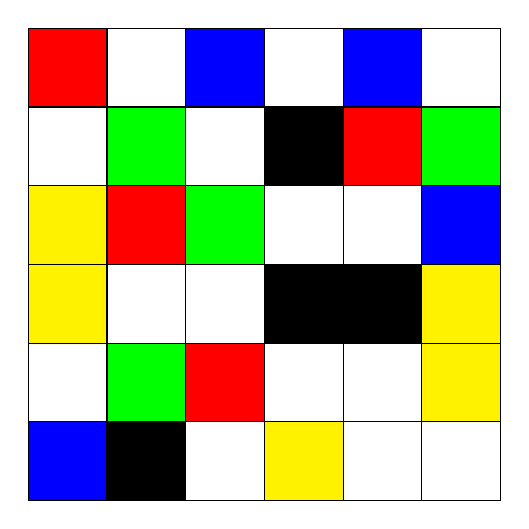
\begin{tikzpicture}
\draw[fill,color=blue] (0,0) rectangle +(1,1);
\draw[fill,color=blue] (4,2) rectangle +(1,1);
\draw[fill,color=blue] (4,5) rectangle +(1,1);
\draw[fill,color=blue] (5,3) rectangle +(1,1);
\draw[fill,color=blue] (2,5) rectangle +(1,1);
\draw[fill,color=black] (1,0) rectangle +(1,1);
\draw[fill,color=black] (3,2) rectangle +(1,1);
\draw[fill,color=black] (4,2) rectangle +(1,1);
\draw[fill,color=black] (3,4) rectangle +(1,1);
\draw[fill,color=yellow] (3,0) rectangle +(1,1);
\draw[fill,color=yellow] (0,2) rectangle +(1,1);
\draw[fill,color=yellow] (5,1) rectangle +(1,1);
\draw[fill,color=yellow] (5,2) rectangle +(1,1);
\draw[fill,color=yellow] (0,3) rectangle +(1,1);
\draw[fill,color=red] (1,3) rectangle +(1,1);
\draw[fill,color=red] (4,4) rectangle +(1,1);
\draw[fill,color=red] (0,5) rectangle +(1,1);
\draw[fill,color=red] (2,1) rectangle +(1,1);
\draw[fill,color=green] (1,1) rectangle +(1,1);
\draw[fill,color=green] (5,4) rectangle +(1,1);
\draw[fill,color=green] (1,4) rectangle +(1,1);
\draw[fill,color=green] (2,3) rectangle +(1,1);
\draw (0,0) grid (6,6);
\end{tikzpicture}
\end{center}

Formal seien $L,N\in \mathbb N$, $L,N\ge 2$. $I\coloneqq\{1,\ldots,N\}^2$, $S\coloneqq \{1,\ldots,L\}^I = \{f:I\to \{1,\ldots,L\}\}$. Sei $(X_n)$ die Markov-Kette in $S$, die die Zustandsfolge angibt.

Wie verhält sich die Folge für $n\to\infty$? Sei $l\in\{1,\ldots,L\}$ fest, und es sei $Y_n$ die Anzahl der Felder mit Farbe $l$ im Zustand $X_n$. Sei $(A,B)$ ein Nachbarpaar im Gitter. Wäre dies die Wahl in einem Zustandsübergang, so gelte: Ist $X_n(A)=X_n(B)$ oder $X_n(A)\ne l, X_n(B)\ne l$, so gilt auch $Y_{n+1}=Y_n$. Ist dagegen $X_n(A)=l$ und $X_n(B)\ne l$, so ist $Y_{n+1}=Y_n-1$. Ist letzlich $X_n(A)\ne l$ und $X_n(B) =l$, so ist $Y_{n+1}=Y_n+1$.

Die Wahrscheinlichkeit, erst $A$, dann $B$ zu wählen ist gleich der Wahrscheinlichkeit, erst $B$ und dann $A$ zu wählen. Damit ist
\[
E[Y_{n+1} \mid X_1,\ldots,X_n] = Y_n
\]
Sei $\mathcal F_n \coloneqq \sigma(X_0,\ldots,X_n)$. Dann ist $(Y_n)_{n\in\mathbb N_0}$ ein $(\mathcal F_n)$-Martingal. Nach der Bemerkung folgt: $Y_n\to Y_\infty$ für ein $n\to\infty$ $P$-fast-sicher. Da $(Y_n)$ ganzzahlig, ist $Y_n(\omega)$ konstant ab einem $n\ge n_0(\omega)$. Als Konstanten kommen nur $0$ und $N^2$ in Frage, denn für $k\in \{1,\ldots,N^2-1\}$ gilt
\begin{align*}
P(Y_{n+j} = k \mid Y_n = \ldots = Y_{n+j-1} = k) &\le 1 - \frac1{N^24} \\
\implies P(Y_n = \ldots = Y_{n+j} = k) &\le (1-\frac1{N^24})^j \\
\implies P(\underbrace{Y_m = k,\, \forall m\ge n}_{\eqqcolon A_n}) &= 0
\end{align*}
Es gilt $\{\omega \in \Omega \mid \exists n\ \forall m\ge n: Y_m(\omega)=k\} = \bigcup_{n=0}^\infty A_n$. Damit ist \[
P(\lim_{n\to\infty} Y_n=k) = P(\exists n\ \forall m\ge n: Y_n=k) \le \sum_{n=0}^\infty P(A_n) =0
\]
und wir folgern dass $P(Y_\infty \in \{0,N^2\}) = 1$.

Außerdem gilt noch, da $Y_n$ beschränkt sind:
\begin{align*}
EY_\infty = \lim_{n\to \infty} EY_n = EY_0
\end{align*}
Damit ist die Wahrscheinlichkeit, dass das Feld irgendwann komplett blau ist, gleich 
\begin{align*}
P(Y_\infty =N^2)=\frac 1{N^2} EY_\infty = \frac 1{N^2}EY_0 = \frac1{N^2}\#\{A\in I\mid X_0(A)=l\}.
\end{align*}

Anwendungen dieses Modells findet man in der Physik (Vielteilchensysteme), in der Biologie (Ausbreitung von Infektionen) oder in der Finanzmathematik (Kreditrisiken).
\end{beispiel}

\section{Die starke Markov-Eigenschaft}

Gegeben si eine Markov-Kette $(X_n)_{n\in\mathbb N_0}$ mit Zustandsraum $S$ auf dem Wahrscheinlichkeitsraum $(\Omega = S_0^{\mathbb N_0}, \mathcal F\da \otimes_{n=0}^\infty \mathcal P(S), P)$. Beachte, dass die Mengen
\begin{align*}
Z(i_0,i_1,\ldots,i_n) \coloneqq \{i_0\} \times \{i_1\} \times \cdots \times \{i_n\} \times S \times S \times \cdots
\end{align*}
für $n\in \mathbb N_0$, $i_0,\ldots i_n\in S$ ein durchschnittstabiles Erzeugendensystem für $\mathcal F$ bilden. Weiter sei $\mathcal (F_n)_{n\in \mathbb N_0}$ mit $\mathcal F_n=\sigma(X_0,\ldots,X_n)$ die natürliche Filtration von $(X_n)$.

$\tau:\Omega \to \mathbb N_0$ sei eine $(\mathcal F_n)$-Stoppzeit\index{Stoppzeit}, das heißt $\{\tau \le n\} \in \mathcal F_n$ und $P(\tau <\infty) = 1$. Die gestoppte Markov-Kette $X^\tau=(X_n^\tau)_{n\in\mathbb N_0}$ ist
\begin{align*}
X_n^\tau \da X_{\min(\tau,n)}
\end{align*}
für $n\in \mathbb N_0$ und $Y=(Y_n)_{n\in\mathbb N_0}$ definiert durch
\begin{align*}
Y_n \da X_{\tau + n}
\end{align*}
heißt der Post-$\tau$-Prozess.\index{Post-$\tau$-Prozess}

\begin{satz}[Starke Markov Eigenschaft]
  \label{Satz6.1}
  Mit den oben eingeführten Bezeichnungen gilt:
  \begin{enuma}
  \item $Y$ ist eine Markov-Kette mit Übergangsmatrix $P$ 
    und Startverteilung $\nu$, wobei $X_\tau\backsim\nu$.
  \item $X^\tau$ und $Y$ sind unter $X_\tau$ bedingt unabhängig.
  \end{enuma}
\end{satz}

\begin{beweis}
  a.) Es gilt:
  \begin{align*}
    & P(Y_0,\dots,Y_n=i_n,Y_{n+1}=i_{n+1}) \\
    = & \sum_{k=0}^\infty P(\tau=k,X_k=i_0,\dots,X_{k+n+1}=i_{n+1}) \\
    = & \sum_{k=0}^\infty P(X_{k+n+1} \vert X_k=i_0,\dots,X_{k+n}=i_n,\tau=k) 
    \cdot P(X_k=i_0,\dots,X_{k+n}=i_n,\tau=k) \\
    = & p_{i_n i_{n+1}} \sum_{k=0}^\infty P(X_k=i_0,\dots,X_{k+n}=i_n,\tau=k) \\
    = & p_{i_n i_{n+1}} P(Y_0=i_0,\dots,Y_n=i_n) \implies \text{ Behauptung}.
  \end{align*}
  b.) Seien
  \begin{align*}
    & A:=Z(i_0,\dots,i_m)={i_0}\times\dots\times {i_m}\times S\times S \times\dots \\
    & B:=Z(j_0,\dots,j_n)
  \end{align*}
  dann gilt:
  \begin{align*}
    & P(X^\tau\in A,Y\in B,X_\tau =j) \\
    =& \sum_{k=0}^\infty P(\tau=k,X_{0\wedge k}=i_0,\dots,X_{m\wedge k}=i_m,
    X_k=j_0,\dots,X_{k+n}=j_n,X_k=j) \\
    =& \sum_{k=0}^\infty P(X_k=j_0,\dots,X_{k+n}=j_n\vert 
    X_{0\wedge k}=i_0,\dots,X_{m\wedge k}=i_m,X_k=j,\tau=k) \\
    & \quad \cdot P(X_{0\wedge k}=i_0,\dots,X_{m\wedge k}=i_m,x_k=j,\tau=k) \\
    =& P(X_0=j_0,\dots,X_n=j_n\vert X_0=j) \cdot P(X^\tau \in A, X_\tau=j) \\
    =& P(Y\in B\vert X_j=j) \cdot P(X^\tau\in A\vert X_\tau=j) \cdot P(X_\tau=j) 
  \end{align*}
  Teilen durch $P(X_\tau=j) \implies$ Behauptung.
\end{beweis}

\chapter{Markov-Ketten in stetiger Zeit}

\section{Ein wichtiger Spezialfall: der Poisson-Prozess}

Gegeben sei ein Wahrscheinlichkeitsraum $(\Omega,\cF,P)$.
Wir betrachten jetzt einen stochastischen Prozess $N=(N_t)_{t\geq 0}$
mit Zustandsraum $\mathbb{N}_0$, d.h. $(N_t)_{t\geq 0}$ ist eine Familie von
$(\cF,\mathcal{P}(\mathbb{N}_0))$-messbaren ZV, der bestimmte Ereignisse zählen soll
(z.B. Emission von Partikeln beim radioaktiven Zerfall, Ankünfte von Kunden in einem
Bediensystem, Schäden bei einer Versicherung). \\
Wir nehmen an, dass mindestens ein Ereignis eintritt und die Anzahl der Ereignisse in einem
kompakten Intervall soll endlich sein. \\
Wir stellen folgende Forderungen an $N$:
\begin{enumerate}[\hspace{1em}{(A}1)]
\item Alle Pfade $t \mapsto N(t,\omega)$ liegen in
\[
D_0:=\{f:[0,\infty)\longrightarrow\mathbb{N}_0\vert f(0)=0,f\uparrow,f \text{ stetig von rechts }\}
\]
%\emph{Hier fehlt ein Bild}
\item $(N_t)_{t\geq 0}$ hat unabhängige Zuwächse, d.h. für alle 
$0\leq t_0\leq t_1 \leq \dots \leq t_n, n\in \mathbb{N}$ sind die ZV
\[
N_{t_0},N_{t_1}-N_{t_0},\dots,N_{t_n}-N_{t_{n-1}}
\]
stochastisch unabhängig.
\item $(N_t)_{t\geq 0}$ hat stationäre Zuwächse, d.h. $\forall t>0$ hängt die Verteilung
von $N_{s+t}-N_s$ nicht von s ab.
\item Ereignisse treten einzeln auf, d.h. $P(N_h\geq2)=o(h)$ mit $h\downarrow 0$.
\end{enumerate}
\begin{bemerkung}
  Der stochastische Prozess kann als Zufallsgröße mit Werten in einem
  Funktionenraum aufgefasst werden, d.h.
  \[
  \Omega\ni\omega\mapsto N(\cdot,\omega)\in D_0
  \]
  Als $\sigma$-Algebra auf $D_0$ wählen wir 
  \[
  \mathfrak L(D_0):=\sigma(\{\pi_t:t\geq 0\})
  \]
  wobei $\pi_t:D_0\longrightarrow\mathbb{N}_0,f\mapsto f(t)$ die $t$-te Projektion ist. \\
  Es gilt: $N_t:\Omega\longrightarrow D_0$ ist $(\cF,\mathfrak Le(D_0))$-messbar 
  $\Longleftrightarrow N_t:\Omega\longrightarrow\mathbb{N}_0$ sind 
  $(\cF,\mathcal P(\mathbb N_0))$-messbar $\forall t\geq0$. 
  (Stochastik II Übungsaufgabe 21) \\
  Die Mengen der Form
  \[
  A(t_1,\dots,t_n,i_1,\dots,i_n):=\{f\in D_0\vert f(t_j)-f(t_{j-1})=i_j \text{ für } f=1,\dots,n\}
  \]
  mit $0=:t_0\leq t_1\leq\dots\leq t_n\leq\infty,i_1,\dots,i_n\in\mathbb N$ 
  bilden ein durchschnittstabiles Erzeugendensystem von $\mathfrak L(D_0)$.
\end{bemerkung}

\begin{satz}
  \label{satz:7.1}
  Es sei $(N_t)_{t\geq 0}$ ein stochastischer Prozess, der den Bedingungen (A1)-(A4) genügt.
  Dann hat $N$ mit Wahrscheinlichkeit $1$ nur Sprünge der Höhe $1$ und es existiert ein
  $\lambda>0$, so dass:
  \begin{enuma}
  \item $\forall s,t\geq 0$ ist $N_{s+t}-N_s$ Poisson-verteilt mit Parameter $\lambda t$.
  \item Die Zeiten zwischen aufeinanderfolgenden Sprüngen des Protesses sind unabhängig und exponentialverteilt mit Parameter $\lambda$.
  \end{enuma}
\end{satz}


\begin{beweis} 
\textbf{Sprünge der Höhe 1:} Es ist also zu zeigen:
  \[
  P(N_s-N_{s-}\geq 2 \text{ für ein } s>0)=0
  \]
  wobei $N_{s-}$ der linksseitige Grenzwert ist. \\
  Für festes $t>0$ gilt:
  \begin{align*}
   & P(N_s-N_{s-}\geq 2 \text{ für ein } s\in (0,t]) \\
\leq \, & P(N_{\frac{kt}{n}}-N_{\frac{(k-1)t}{n}}\geq 2 \text{ für ein } k\in\{1,\dots,n\} \\    
\leq \, & n\cdot P(N_{\frac{t}{n}}\geq 2)
  \end{align*}

(das letzte $\leq$ gilt wegen (A3)) \\
Aus (A4) folgt:
\[
\lim_{n\rightarrow\infty} \frac{P(N_{\frac{t}{n}}\geq 2)}{\frac{t}{n}}\cdot t=0
\]
Weiter gilt mit Stetigkeit des Wahrscheinlichkeitsmaßes:
\[
P(N_s-N_{s-}\geq 2 \text{ für ein } s>0)=
\lim_{t\rightarrow\infty}P(N_s-N_{s-}\geq 2 \text{ für ein } s\in (0,t])=0
\]

\textbf{a)} Betrachte dazu
\[
\Phi:[0,\infty) \to [0,1] \text{ mit }\Phi(t) \da P(N_t =0).
\]
Für alle $s,t>0$ folgt:
\begin{align*}
\Phi(s+t)
&= P(N_s = 0,N_{s+t} - N_s = 0) \\
 &= P(N_s=0) \cdot P(N_t=0) &\text{(nach (A3) und (A2))}\\
&= \Phi(s) \cdot \Phi(t)
\end{align*}
Daraus folgt, dass $\Phi(\frac kn) = (\Phi(\frac 1n))^k$ und $\Phi(1) = \Phi(\frac 1n + \cdots \frac 1n) = (\Phi(\frac 1n))^n$ für $k,n\in \MdN$ gilt. Das heißt, dass $\Phi(\frac kn) = (\Phi(1))^{\frac kn}$.

Da $\Phi$ fallend ist folgt mit einem Einschachtelungsargument: 
\[
\Phi(t) = (\Phi(1))^t\text{ für alle } t >0
\]
Weiter ist $\Phi(1) \in (0,1)$, da $\Phi(1) \in[0,1]$ und falls $\Phi(1)=1$, dann wäre 
\[
P(N_t = 0 \text{ für alle } t\ge 0)= \lim_{t\to\infty} \phi(t) = 1
\]
im Widerspruch zur Forderung, dass mindestens ein Ereignis eintritt, und wäre $\Phi(1) = 0$, dann gälte für alle $n\in \MdN$
\begin{align*}
P(N_1\ge u) 
&\ge P(N_{\frac kn} - N_{\frac {k-1}n} \ge 1 \text{ für } k =1,\ldots,n)\\
&= \Big(1-\Phi(\frac 1n)\Big) ^n &\text{((A2), (A3))} \\
&= 1
\end{align*}
im Widerspruch zur Forderung, dass in kompakten Intervallen nur endlich viele Ereignisse eintreten.

Sei jetzt 
\[
\lambda \da - \log \Phi(1).
\]
Es ist $0<\lambda <\infty$ und $P(N_t=0)= (\Phi(1))^t = e^{-\lambda t}$. Weiter sei $t>0$ und für $n\in \MdN$ definieren wir
\begin{align*}
X_{nk} &\da 1_{\MdN}\big(N_{\frac{kt}n} - N_{\frac{(k-1)t}n}\big)\\
&= 
\begin{cases}
1, &\text{falls mindestens ein Ereignis in $\big(\frac{kt}n, \frac{(k-1)t}n\big]$ eintritt}\\
0, &\text{sonst}
\end{cases}
\end{align*}
Wegen (A2) sind die $X_{n1},\ldots,X_{nn}$ unabhängig und wegen (A3) identisch verteilt mit $B(1,1-e^{-\lambda \frac tn})$. Dann gilt
\begin{align*}
\sum_{k=1}^n X_{nk} \sim B(n,1-e^{-\lambda \frac tn}) \tomit d \operatorname{Po}(\lambda t)
\end{align*}
da $n(1-e^{-\lambda \frac tn}) \tomit{n\to \infty} \lambda t$.

Aus (A4) folgt:
\begin{align*}
P(\sum_{k=1}^n X_{nk} \ne N_t) 
&= P(\bigcup_{k=1}^n\{N_{\frac {kt}n} - N_{ \frac{(k-1)t}n} \ge 2\})\\
&\le n \cdot P(N_{\frac tn} \ge 2) \tomit {n\to \infty} 0
\end{align*}
und damit haben wir gezeigt, dass
\[
N_t \sim \operatorname{Po}(\lambda t).
\]

\textbf{b)} Sei
\[
T_1 \da \inf \{t>0\mid N_t \ne 0\}
\]
der erste Sprungzeitpunkt. Wir erhalten
\begin{align*}
P(T_1 > t) = P(N_t = 0) = e^{-\lambda t}\text{ mit } t \ge 0
\end{align*} und damit
\[
T_1 \sim \exp(\lambda).
\]
Die weiteren Aussagen werden später gezeigt.
\end{beweis}


\begin{bemerkung}
Der Prozess $N=(N_t)_{t\ge 0}$ in Satz \ref{satz:7.1} heißt \emph{Poisson-Prozess}\index{Poisson-Prozess} mit Parameter $\lambda$.
\end{bemerkung}

Die Bedinungen (A2) und (A3) können etwas „abstrakter“ gefasst werden: Für $u\ge 0$ definiere
\begin{align*}
S_u &: D_0 \to D_0,  & f &\mapsto f(\cdot\wedge u)\\
Z_u &: D_0 \to D_0,  & f &\mapsto f(u+\cdot)-f(u)
\end{align*}
wobei $(\cdot \wedge u)$ die Abbildung $v\mapsto \min (v,u)$ darstellt.

Beide Abbildungen sind $(\frak L(D_0), \frak L(D_0))$-messbar.

Wir können also auch stochastische Prozesse $S_u(N) = (N_{t\wedge u})_{t\ge 0}$ und $Z_u(N) = (N_{u+t} - N_n)_{t\ge 0}$ als Zufallsgröße mit Werten in $(D_0,\mathfrak L(D_0))$ auffassen.

Weiter gilt mit 
\[
A(t_1,\ldots,t_n;i_1,\ldots,i_n) \da \{f\in D_0\mid f(t_j) - f(t_{j-1}) = i_j\text{ für }j=1,\ldots,n\},
\]
wobei $0 \ad t_0\le t_1\le \cdots\le t_n < \infty$, $i_1,\ldots,i_n\in\MdN_0$, dass
\[
\{S_u(N) \in A(t_1,\ldots,t_n;i_1,\ldots,i_n)\} 
= \{ N_{t_1\wedge u}- N_{t_0\wedge u} = i_1,\ldots,N_{t_n\wedge u}- N_{t_{k-1}\wedge u} = i_k\}
\]
und
\[
\{Z_u(N) \in A(s_1,\ldots,s_l;j_1,\ldots,j_l)\} 
= \{ N_{n+s_1}- N_{n+s_0} = j_1,\ldots,N_{n+s_l}- N_{n+s_{l-1}} = j_k\} 
\]
Wegen (A2) folgt:
\begin{multline*}
P\big(S_u(N) \in A(t_1,\ldots,t_n;i_1,\ldots,i_n),\,
 Z_u(N) \in A(s_1,\ldots,s_l;j_1,\ldots,j_l)\big) \\
= P\big(S_u(N) \in A(t_1,\ldots,t_n;i_1,\ldots,i_n)\big) 
\cdot P\big(Z_u(N) \in A(s_1,\ldots,s_l;j_1,\ldots,j_l)\big) 
\end{multline*}
und daraus die Unahbhängigkeit der Prozesse $S_u(N)$ und $Z_u(N)$.

Analog folgt:
\[
P\big(Z_u(N) \in A(s_1,\ldots,s_l;j_1,\ldots,j_l)\big) 
= P\big( N \in A(s_1,\ldots,s_l;j_1,\ldots,j_l)\big)
\]
Also haben $Z_u(N)$ und $N$ dieselbe Verteilung.

Diese Aussagen können jetzt auf Stoppzeiten verallgemeinert werden. Es sei dazu $\mathcal F_t \da \sigma(\{N_s, s\le t\})$ für $t\ge 0$ und $(\mathcal F_t)_{t\ge 0}$ die natürliche Filtration.

\begin{definition}
Sei $\tau$ eine $(\mathcal F_t)_{t\ge 0}$-Stopptzeit\index{Stoppzeit}, das heißt $\{\tau \le t \} \in \mathcal F_t$. Der Prozess 
\[
S_\tau(N) = (N_{\tau \wedge t})_{t\ge 0}
\]
heißt \emph{Prä-$\tau$-Prozess}\index{Prä-$\tau$-Prozess} und der Prozess 
\[
Z_\tau(N) = (N_{\tau + t} - N_\tau)_{t \ge 0}
\]
heißt \emph{Post-$\tau$-Prozess}\index{Post-$\tau$-Prozess}.
\end{definition}

\begin{lemma}
\label{lem:7.2}
Ist $\tau$ eine endliche Stoppzeit, so sind die Prozesse $(N_{\tau \wedge t})_{t\ge 0}$ und $(N_{\tau + t}-N_\tau)_{t\ge 0}$ stochastisch unabhängig. Außerdem hat $(N_{\tau + t}-N_\tau)_{t\ge 0}$ dieselbe Verteilung wie $(N_t)_{t\ge 0}$.
\end{lemma}

\begin{beweis}
Zunächst nehmen wir an, dass $\tau$ Werte in $\mathbb Q_+$ annimmt. Für $0\le s_1\le\cdots\le s_k$, $0\le t_1\le \cdots\le t_l$ und beliebige $i_1,\ldots,i_k,j_1,\ldots,j_k\in \mathbb N_0$ gilt
\begin{align*}
C&\da P\big(S_\tau(N) \in \underbrace{A(s_1,\ldots,s_k;i_1,\ldots,s_k)}_{\ad A},\,
Z_\tau(N) \in \underbrace{A(t_1,\ldots,t_l;j_1,\ldots,j_l)}_{\ad B}
\big) \\
&= \sum_{u\in \mathbb Q_+} P(\tau = u,\, S_u(N)\in A,\, Z_u(N)\in B)\\
\intertext{Da $\{\tau = u \} \in \cF_u$ kann dieses Ereignis durch $S_u(N)$ ausgedrückt werden. Da $S_u(N)$ und $Z_u(N)$ unabhängig sind, folgt:
}
\cdots &= \sum_{u\in\mathbb Q_+} P(\tau = u, S_u(N)) \cdot P(\underbrace{Z_u(N)\in B}_{= N\in B}) \\
&= P(N\in B) \cdot P(S_\tau(N) \in A)
\end{align*}
Im Fall $k=1,s_1=0,i_1=0$ folgt:
\begin{align*}
P(Z_\tau(N)\in B) = P(N\in B)
\end{align*}
also gilt $Z_\tau(N) \gleichnach{d} N$ und damit
\begin{align*}
P(S_\tau (N) \in A,\, Z_\tau(N)\in B) = P(Z_\tau (N) \in B) \cdot P(S_\tau(N)\in A)
\end{align*}
also sind $Z_\tau(N)$ und $S_\tau(N)$ unabhängig.

Weiter sei $\tau$ beliebig. Betrachte die Folge 
\[
\tau_n \da \frac{\lceil 2^n \tau \rceil}{2^n},\, n\in \mathbb N,
\]
für die $\tau_n\in \mathbb Q_+$ $P$-fast-sicher gilt und $\tau_n\to \tau$ für $n\to\infty$. Mit (A1) folgt für alle $t\ge 0$
\[
N_{\tau_n\wedge t} \tomit{n\to\infty} N_{\tau \wedge t},\quad N_{\tau_n+t}\tomit{n\to\infty}N_{\tau+t}
\]
$P$-fast-sicher und
\begin{align*}
P(S_\tau(N)\in A,\, Z_\tau(N)\in B) 
&= \lim_{n\to\infty} P(S_{\tau_n}(N)\in A,\, Z_{\tau_n}(N)\in B) \\
&= \lim_{n\to\infty} P(S_{\tau_n}(n)\in A) \cdot P(Z_{\tau_n}(N)\in B)\\
&= P(S_\tau(N)\in A)\cdot P(Z_\tau(N)\in B)
\end{align*}

Analog kann man die Aussage $Z_\tau(N)\gleichnach{d}N$ auf beliebige $\tau$ erweitern.
\end{beweis}

Damit können wir den Beweise von Satz $\ref{satz:7.1}$ abschließen:

Es seien
\begin{align*}
T_1 &\da \inf\{t>0\mid N_t\ne 0\} \\
S_1 &\da T_1 \\
S_k &\da \inf\{t>S_{k-1} \mid N_t \ne T_{t-}\},\ k=2,3,\ldots\\
T_k &\da S_k - S_{k-1},\ k=2,3,\dots
\end{align*}
Wir wissen bereits, dass $T_1 \sim \exp(\lambda)$. Induktiv nehmen wir dann, dass $T_1,\ldots,T_k$ unabhängig und identisch exponential-verteilt seien. $\tau \da T_1 + \cdots + T_k = S_k$ ist eine Stoppzeit, da $\{\tau \le t\} = \{N_t \ge k\} \in \cF_t$. Da $P(\tau > t)= P(N_t < k) \to 0$ für $t\to\infty$ gilt, ist $\tau$ $P$-fast-sicher endlich.

$T_{k+1}$ ist die Zeit bis zum ersten Sprung im Post-$\tau$-Prozess. Nach Lemma $\ref{lem:7.2}$ ist $T_{k+1}\gleichnach{d} T_1\sim \exp(\lambda)$ und $T_{k+1}$ ist unabhängig von $S_\tau(N)$, also auch von $T_1,\ldots,T_k$.

\begin{beispiel}[Bedingte Gleichverteilungseigenschaft]
Es seien $K,X_1,X_2,\ldots$ unabhängige Zufallsvariablen mit $K\sim \operatorname{Po}(\lambda T)$, $T>0$, und $X_i\sim U(0,T)$.

Wir definieren\[
N_t \da \#\{1\le i \le K\mid X_i\le t\},\, t\ge 0.
\]
Es sei $0\ad t_0\le t_1 \le \cdots\le t_n=T$ eine Zerlegung des Intervals $[0,T]$. Betrachte für $i_1,\ldots,i_n\in \mathbb N_0$ das Ereignis
\[
A \da \{N_{t_1} - N_{t_0} = i_1,\ldots,N_{t_n}-N_{t_{n_1}} = i_n\}.
\]
Für $\omega \in A$ folgt $k \da K(\omega) = i_1+\cdots+ i_n$. Man erhält (siehe Definition der Multinomialveteilung, Henze, Stochastik I, S. 121)
\begin{align*}
P(N_{t_1} - N_{t_0}=1,\ldots,N_{t_n} - N_{t_{n-1}} = i_n) 
&= e^{-\lambda T}\frac{(\lambda T)^k}{k!} \frac{k!}{i_1!\cdots i_n!}\Big(\frac{t_1\cdot t_0}{T}\Big)^{i_1}\cdots \Big(\frac{t_n\cdot t_{n-1}}{T}\Big)^{i_n} \\
&= \prod_{l=1}^n \underbrace{e^{-\lambda(t_l-t_{l-1})} \frac{(\lambda (t_l - t_{l-1}))^{i_l}}{i_l!}}_{=P(M_l=i_l)}
\end{align*}
wobei $M_l\sim \operatorname{Po}(\lambda(t_l-t_{l-1}))$. Das zeigt: Die Zuwächse des Prozesses $\tilde N=(N_t)_{0\le t\le T}$ sind unabhängig und stationär und Poisson-verteilt mit Parameter $\lambda\cdot$Intervalllänge, und (A1), (A4) ist erfüllt, also ist $\tilde n$ ein bei $T$ gestoppter Poisson-Prozess.
\end{beispiel}

\begin{beispiel}[Das Inspektions-Paradox]
Es seien $X_1,X_2,\ldots$ unabhängig und identisch verteilte Zuvallsvariablen mit $X_k\sim \exp(\lambda)$, welche die Lebensdauer von Glühbirnen modellieren.

Es sei $S_n \da \sum_{k=1}^n X_k$ der Zeitpunkt, an dem die $n$-te Birne kaputt geht und eine neue Birne eingesetzt wird, und $N_t$ die Anzahl der Erneuerungen bis zum Zeitpunkt $t$ und damit ein Poisson-Prozess mit Parameter $\lambda$.

In der Erneuerungstheorie interessiert man sich für 
\begin{align*}
V_t &\da S_{N_t+1}-t = \text{Restlebensdauer} \\
W_t &\da t- S_{N_t} = \text{Alter} \\
L_t &\da  W_t + V_t = \text{Gesamtlebensdauer}
\end{align*}
der zum Zeitpunkt $t$ in Gebrauch befindlichen Glühbirne.

Es ist $V_t \sim \exp(\lambda)$, da die Exponentialverteilung gedächtnislos ist. Die Variable $W_t$ kann höchstens $t$ sein, das heißt $P(W_t > s) = 0$ für $s>t$. Für $0\le s \le t$ gilt $P(W_t \ge s) = P(N_t-N_{t-s} = 0) = e^{-\lambda s}$. Damit ist
\begin{align*}
F_{W_t}(s) = 
\begin{cases}
1-e^{-\lambda s},& 0\le s \le t \\
1, & s\ge t.
\end{cases}
\end{align*}
Außerdem sind nach der starken Markoveigenschaft die Zufallsvariablen $W_t$ und $V_t$ unabhängig. $L_t$ ergibt sich als Faltung dieser Variablen. Die Dichte $F_{L_t}$ für $s\ge t$:
\begin{align*}
f_{L_t}(s) &= \int_0^s f_{V_t}(s-u)F_{W_t}(du) \\
&= \int_0^t \lambda e^{-\lambda(s-u)}\lambda e^{-\lambda} du + \lambda e^{-\lambda(s-t)}\cdot e^{-\lambda t} \\
&= \lambda (1+\lambda t)e^{-\lambda s}\\
\intertext{und für $s < t$:}
f_{L_t}(s) &= \int_0^s \lambda e^{-\lambda(s-u)}\lambda ^{-\lambda u}du \\
&= \lambda ^2 s e^{-\lambda s}
\end{align*}
Also ist $L_t$ \emph{nicht} $\exp(\lambda)$-verteilt! Für großes $t$ gilt
\[
EL_{t} \approx 2 EX_i=\frac 2 {\lambda}.
\]
Dieses Ergebnis lässt sich sich erklären: Inspiziert man zu einer zufälligen Zeit die aktuell leuchtende Glühbirne, so ist die Wahrscheinlichkeit, eine länger lebende zu erwischen, größer, als eine kurzlebige Birne anzutreffen.
\end{beispiel}

\section{Der allgemeine Fall im Schnelldurchgang}

\begin{definition}
Ein stochastischer Prozess $(X_t)_{t\ge 0}$ mit abzählbarem Zustandsraum $S$ heißt (homogene) Markov-Kette,\index{Markov-Kette!zeitstetig} falls gilt:
Für alle $n\in\mathbb N$ und $0\le t_0 < t_1 < \cdots < t_n$, $t,h>0$ und $i_k\in S$ mit $P(X_{t_k}=i_k,\, 0\le k\le n) > 0$:
\begin{align*}
P(X_{t_n+h}=i_{n+1} \mid X_{t_k}=i_k,\, 0\le k\le n) &= P(X_{t_n+k} = i_{k+1} \mid X_{t_n} = i_n) \\ 
&= P(X_{t+h} = i_{n+1} \mid X_t=i_n)
\end{align*}
\end{definition}

\begin{bemerkung}
Definieren wir für alle $i,j\in S$
\[
P_{ij}(t) \da P(X_t = j \mid X_0 = i)
\]
und die Matrix
\[
P(t) = \big(p_{ij}(t)\big)_{i,j\in S}
\]
so gelten analog zum diskreten Fall die Chapman-Kolmogorov-Gleichungen für alle $i,j\in S$, $s,t>0$:\index{Chapman-Kolmogorov-Gleichungen}
\[
p_{ij}(t+s) = \sum_{k\in S} p_{ik}(t) p_{kj}(s)
\]
Mit $P(0)=E$ wird $\{P(t): t\ge 0\}$ zu einer Halbgruppe von stochastischen Matritzen. Diese nennen wir \emph{Übergangsmatritzenfunktion}\index{Übergangsmatritzenfunktion}.

Falls zusätzlich für $i,j\in S$ 
\[
\lim_{t\downarrow 0} p_{ij}(t)=\delta_{ij}
\]
gilt, also $P(t)$ rechtseitig stetig ist, dann heißt sie \emph{Standardübergangsmatritzenfunktion}\index{Standardübergangsmatritzenfunktion}.
\end{bemerkung}


\begin{satzunddefinition}
Sei $\{P(t): t\ge 0\}$ eine Standardübergangsmatritzenfunktion. Dann ist jedes $p_{ij}(t)$ in 0 rechtseitig differenzierbar, das heißt es existiert für alle $i,j\in S$
\[
q_{ij} \da \lim_{t\downarrow 0} \frac 1t (p_{ij}(t) - \delta_{ij}).
\]
Die Matrix $Q\da (q_{ij})$ heißt \emph{Intensitätsmatrix}\index{Intensitätsmatrix} oder \emph{infinitesimaler Erzeuger}\index{infinitesimaler Erzeuger} (Generator) zu $\{P(t): t\ge 0\}$.
\end{satzunddefinition}

\begin{beispiel}
Es sei $N=(N_t)_{t\ge 0}$ ein Poisson-Prozess mit Itensität $\lambda$. Dann gilt für $i_{n+1}\ge i_n$:
\begin{align*}
P(N_{t_{n+1}} = i_{n+1} \mid N_{t_0} = i_0 ,\ldots,N_{t_n}=i_n)
&= P(N_{t_{n+1}} - N_{t_n} = i_{n+1} - i_n)\\
&= e^{-\lambda (t_{n+1}-t_n)}\frac{(\lambda(t_{n+1}-t_n))^{i_{n+1}-i_n}}{(i_{n+1}-i_n)!}
\end{align*}
Also ist $N$ eine homogene Markov-Kette mit Übergangsmatrix
\[
p_{ij}(t) = 
\begin{cases}
e^{-\lambda t}\frac{(\lambda t)^{j-i}}{(j-i)!}, &\text{falls }j\ge i \\
0,&\text{sonst}
\end{cases}
\]
weiter gilt 
\begin{align*}
\lim_{t\downarrow 0} \frac 1t(p_{ij}(t) - \delta_{ij}) =
\begin{cases}
\phantom{-}\lambda,&\text{falls }j=i+1 \\
-\lambda, &\text{falls }j=i \\
\phantom{-}0, &\text{sonst.}
\end{cases}
\end{align*}
\end{beispiel}

\begin{lemma}
Sei $\{P(t):t\ge 0\}$ eine Standardübergangsmatritzenfunktion. Dann gilt für $q_{ij} \da p_{ij}'(0)$:
\begin{enuma}
\item $0\le q_{ij} < \infty$, $i\ne j$, $-\infty \le  q_{ii} \le 0$.
\item $\sum_{j\ne i} q_{ij} \le -q_{ii} \ad q_i$. Falls $S$ endlich ist, gilt für alle $i\in S$: $q_i = \sum_{j\ne i} q_{ij}$. In diesem Fall heißt die Standardübergangsmatritzenfunktion \emph{konservativ}\index{konservativ}.
\end{enuma}
\end{lemma}

\begin{beweis}
\begin{enuma}
\item $0\le q_{ij}$ für $i\ne j$ und $q_{ii} \le 0$ klar, da $0\le p_{ij} \le 1$. Schwieriger ist zu zeigen, dass $p_{ij}<\infty$, hier wird auf die Literatur verwiesen.
\item  Es gilt für $t\ge 0$:
\begin{align*}
\sum_{i\ne j} \frac {p_{ij}(t)}t &= \frac{1-p_{ii}(t)}t 
\end{align*}
und damit mit Fatour
\begin{align*}
-q_{tt} = \lim_{t\downarrow 0}  \frac{1-p_{ii}(t)}t 
\ge \sum_{i\ne j} \limsup_{t\downarrow 0} \frac{p_{ij}(t)}{t} = \sum_{i\ne j} q_{ij}
\end{align*}
und Gleichheit für endliche $S$.
\end{enuma}
\end{beweis}

\begin{satz}
\label{satz:8.3}
Sei $\{P(t) : t\ge 0\}$ eine Standardübergangsmatritzenfunktion und $S$ sei endlich. Dann gilt das sogenannte \emph{Kolmogorovsche Rückwärtsdifferentialgleichungssystem}\index{Kolmogorovsche Rückwärts-DGL}: Für $t\ge 0$ ist
\begin{align*}
P'(t) = QP(t)
\end{align*}
das heißt für alle $i,j\in S$ ist
\begin{align*}
p_{ij}'(t) = -q_i p_{ij}(t) + \sum_{k\ne i} q_{ik}p_{kj}(t).
\end{align*}
\end{satz}

\begin{beweis}
Wegen Chapman-Kolmogorov gilt für $i,j\in S$, $t,h>0$:
\begin{align*}
p_{ij}(t+h) &= \sum_{k\in S} p_{ik}(h) p_{kj}(t) \\
\implies \frac{p_{ij}(t+h) - p_{ij}(t)}h &=
\frac{p_{ii}(h) - 1}h p_{ij}(t) + \sum_{k\ne i} \frac{p_{ik}(h)}h p_{kj}(t) 
\end{align*}
Für $h\downarrow0$ geht die rechte Seite gegen
\[
-q_i p_{ij}(t) + \sum_{k\ne i}q_{ik}p_{kj}(t)
\]
woraus die Behauptung folgt.
\end{beweis}

\begin{bemerkung}
\begin{enuma}
\item Unter milden Bedingungen ($\{P(t): t\ge 0\}$ eine konservative Standardübergangsmatritzenfunktion und $q_i$ für alle $i\in S$ endlich) gilt Satz \ref{satz:8.3} auch für abzählbares $S$. Weitere Bedinungen sind nötig für das Kolmogorovsche-Vorwärtsdifferentialgleichungssystem
\[
P'(t) = P(t)Q.
\]
\item Falls $S$ endlich ist, ist die Lösung von $P'(t) =QP(t)$, $P(0)=E$ gegeben durch
\[
P(t) =e^{tQ} = \sum_{n=0}^\infty \frac{(tQ)^n}{n!}
\]
\end{enuma}

\end{bemerkung}

\begin{beispiel}
  \begin{align*}
    & S=\{0,1\}, 0<q_0,q_1<\infty \\
    & Q=\left(
    \begin{array}{cc}
      -q_0 & q_0 \\
      q_1 & -q_1 \\
    \end{array}
    \right)
  \end{align*}
  Rückwärts-Differentialgleichung $P'(t)=QP(t)$
  \[
  P(t)=\left(
  \begin{array}{cc}
    p_{00}(t) & p_{01}(t) \\
    p_{10}(t) & p_{11}(t) \\
  \end{array}
  \right)
  \]
  \begin{align*}
   (1) \quad p_{00}'(t)=-q_0p_{00}(t)+q_0p_{10}(t) \\
   (2) \quad p_{01}'(t)=-q_0p_{01}(t)+q_0p_{11}(t) \\
   (3) \quad p_{10}'(t)=-q_1p_{10}(t)+q_1p_{00}(t) \\
   (4) \quad p_{11}'(t)=-q_1p_{11}(t)+q_1p_{01}(t) \\    
  \end{align*}
  Es gilt: $p_{01}(t)=1-p_{00}(t), p_{11}(t)=1-p_{10}(t)$ \\
  Eingesetzt in (2): $-p_{00}'(t)=-q_0+q_0p_{00}(t)+q_0-q_0p_{10}(t)=$ (1) \\
  also ist (2) überflüssig. Analog: (4) ist überflüssig. Sei
  \[
  y(t)=\left(
  \begin{array}{c}
    p_{00}(t) \\ p_{10}(t) \\
  \end{array}
  \right) \]
  Zu lösen: $y'(t)=Qy(t), y(0)=(1,0)^T$. Die Eigenwerte von Q sind:
  $\lambda_1=0, \lambda_2=-(q_0+q_1)$ Eigenvektoren:
  $v_1=\begin{pmatrix} 1 \\ 1 \end{pmatrix}, v_2 =\begin{pmatrix} -q_0 \\ q_1 \end{pmatrix}$
  \[
  \implies y(t)=\alpha\begin{pmatrix} 1 \\ 1\end{pmatrix}+\beta\begin{pmatrix} -q_0 \\ q_1 
  \end{pmatrix} e^{-(q_0+q_1)t}
  \]
  $y(0)=\begin{pmatrix} 1 \\ 0\end{pmatrix}$ liefert $\alpha=\frac{q_1}{q_0+q_1},
  \beta=-\frac{1}{q_0+q_1}$ \\
  Insgesamt also:
  \begin{align*}
    & p_{00}(t)=\frac{q_1}{q_0+q_1}+\frac{q_0}{q_0+q_1}e^{-(q_0+q_1)t} \\
    & p_{10}(t)=\frac{q_1}{q_0+q_1}-\frac{q_1}{q_0+q_1}e^{-(q_0+q_1)t} \\
  \end{align*}
  Hier fehlt ein kleines Bild, das zeigt, wie $p_{00}$ und $p_{10}$ so aussehen. \\
  Wir wollen weiter annehmen, dass die Pfade der Markov-Kette $(X_t)_{t\geq 0}$ in
  \[
  D(s):=\{f:[0,\infty)\longrightarrow S\vert f(t+)=f(t) \ \forall t\geq0,f(t-) \text{ existiert } \forall t>0\}
  \]
  liegen (diskrete Topologie auf $S$). Die Eigenschaft der $f$ in $D(s)$ wird auch mit RCLL oder
  càdlàg bezeichnet. \\
\end{beispiel}
  Gegeben sei jetzt eine Intensitätsmatrix $Q=(q_{ij}),q_{ij}\in\mathbb R$ mit
  (Q1) $q_{ij}\geq0\ \forall i,j\in S, i\neq j, q_{ij}\leq 0 \ \forall i\in S$ \\
  (Q2) $\sum_{j\in S}q_{ij}=0 \ \forall i\in S$ \\
  (Q3) $0<\sup_{i\in S}|q_{ij}|=:\lambda<\infty$ \\
  \begin{satz}
    \label{Satz 8.4}
    Für eine Matrix $Q$ gelte (Q1)-(Q3). Es sei $N=(N_t)_{t\geq0}$ ein Poisson-Prozeß mit
    Intensität $\lambda$ und $Y=(Y_n)_{n\in\mathbb N_0}$ eine von $N$ unabhängige Markov-Kette
    mit Start in $i_0\in S$ und Übergansmatrix $\tilde{P}=(\tilde{p}_{ij})_{i,j\in S},
    \tilde{P}:=E+\frac{1}{\lambda}Q$, also
    \[
    \tilde{p}_{ij}=\delta_{ij}+\frac{q_{ij}}{\lambda} \quad \forall i,j\in S.
    \]
    Dann ist $X=(X_t)_{t\geq0}$ mit $X_t:=Y_{N_t} \quad\forall t\geq0$ eine Markov-Kette
    mit Start in $i_0$, Pfaden in $D(s)$ und Intensitätsmatrix $Q$.
  \end{satz}
  \begin{beweis}
    Offenbar ist $\tilde{P}$ eine stochastische Matrix, $X_0=i_0$ und die Pfade in $D(s)$.
    Für $0\leq t_0<t_1<\dots<t_{n+1}, \ i_0,\dots,i_{n+1}\in S$ gilt:
    \begin{align*}
      & P(X_{t_m}=i_m,0\leq m\leq n+1) \\
      =& \sum_{k_0,\dots,k_{n+1}\in\mathbb N_0} P(N_{t_m}=k_m, Y_{k_m}=i_m, 0\leq m\leq n+1) \\
      =& \sum_{k_0,\dots,k_{n+1}\in\mathbb N_0} P(N_{t_m}=k_m, 0\leq m\leq n+1)\cdot P(Y_{k_m}=i_m, 0\leq m\leq n+1) \\
    \end{align*}
    Betrachte die Faktoren:
    \begin{align*}
      & P(N_{t_m}=k_m, 0\leq m\leq n+1)=P(N_{t_{n+1}}-t_n=k_{n+1}-k_n)\cdot P(N_{t_m}=k_m, 0\leq m \leq n) \\
      & P(Y_{k_m}=i_m, 0\leq m \leq n+1) = P(Y_{k_m}=i_m, 0\leq m \leq n) \cdot \tilde{p}_{i_ni_{n+1}}^{(k_{n+1}-k_n)} \\
    \end{align*}
    Sei jetzt $l:=k_{n+1}-k_n$, dann
    \begin{align*}
      & P(X_{t_m}=i_m, 0\leq m \leq n+1) \\ 
      =& P(X_{t_m}=i_m, 0\leq m \leq n)\cdot \sum_{l=0}^\infty \tilde{p}_{i_ni_{n+1}}^{(l)} \cdot P(N_{t_{n+1}t_n}=l) \\
    \end{align*}
    $\implies X$ ist eine Markov-Kette in stetiger Zeit (und homogen) mit Übergansmatrix:
    \[
    p_{ij}(t)=\sum_{l=0}^\infty\tilde{p}_{ij}^{(l)}e^{-\lambda t} \frac{(\lambda t)^l}{l!}
    \]
    Bestimme Ableitungen $p_{ij}'(0) \ \implies \ Q$ ist wie gewünscht.
  \end{beweis}
  Eine "Umkehrung" des Satzes gilt: \\
  Dazu sei $X=(X_t)_{t\geq 0}$ eine Markov-Kette mit Zustandsraum $S$ und Sprungzeiten: 
  \begin{align*}
    & S_0=0 \\
    & S_1=\inf\{t\geq0\vert X_t\neq X_0\} \\
    & S_n:=\inf\{t>S_{n-1}\vert X_t\neq X_{S_{n-1}} \}, n\geq 2. \\
  \end{align*}
  Verweildauern: $n\geq 1$:
  \[
  T_n:=S_n-S_{n-1}
  \]
  Weiter sei die eingebettete Markov-Kette $Y=(Y_N)$ gegeben durch: $Y_n:=X_{S_n}, n\in\mathbb N_0$.
  \begin{satz}
    \label{satz8.5}
    Es sei $X=(X_t)_{t\geq0}$ eine Markov-Kette mit Zustandsraum $S$ und Intensitätsmatrix $Q$, 
    wobei (Q1)-(Q3) erfüllt seien. \\
    Dann gilt:
    \begin{enuma}
    \item $Y=(Y_n)$ ist eine (zeitdiskrete) Markov-Kette mit Übergansmatrix $P=(p_{ij})$, wobei
      \begin{align*}
	& p_{ij}=\begin{cases}
	\frac{q_{ij}}{q_i} & , \text{ falls } i\neq j \\
	0 & , \text{ falls } i=j
	\end{cases} , \text{ falls } q_i>0 \\
	& p_{ij}=\delta_{ij}, \text{ falls } q_i=0 \\
      \end{align*}
    \item $T_1,T_2,\dots$ sind bedingt unter $(Y_n)$ stochastisch unabhängig mit
      \[
      T_n\sim \exp(q_{Y_{n-1}})
      \]
      Hier fehlt ein Bild.
    \end{enuma}
  \end{satz}

\chapter{Satz um Satz (hüpft der Has)}
\listtheorems{satz,wichtigedefinition}

\renewcommand{\indexname}{Stichwortverzeichnis}
\addtocounter{chapter}{1}
\addcontentsline{toc}{chapter}{\protect\numberline {\thechapter}Stichwortverzeichnis}
\printindex
\end{document}
